%%% LaTeX Template: Two column article
%%%
%%% Source: http://www.howtotex.com/
%%% Feel free to distribute this template, but please keep to referal to http://www.howtotex.com/ here.
%%% Date: February 2011

%%% Preamble
\documentclass[	DIV=calc,%
				paper=a4,%
				fontsize=9pt,%
				onecolumn]{scrartcl}	 					% KOMA-article class

\usepackage{lipsum}													% Package to create dummy text



\usepackage[english]{babel}										% English language/hyphenation
\usepackage[protrusion=true,expansion=true]{microtype}				% Better typography
\usepackage{amsmath,amsfonts,amsthm}					% Math packages
\usepackage[pdftex]{graphicx}						% Enable pdflatex 
%\usepackage[svgnames]{xcolor}									% Enabling colors by their 'svgnames'
\usepackage[hang, small,labelfont=bf,up,textfont=it,up]{caption}	% Custom captions under/above floats
\usepackage{epstopdf}												% Converts .eps to .pdf
\usepackage{subfig}													% Subfigures
\usepackage{booktabs}												% Nicer tables
\usepackage{fix-cm}													% Custom fontsizes

\usepackage[usenames,dvipsnames]{color}
\usepackage{float}
\usepackage{subfig}
%\usepackage{tikz}
\usepackage{acronym}
\usepackage{amsthm}
\usepackage{fancyvrb}
\usepackage{listings}


\usepackage{gitinfo}

% custom changes:
\usepackage[usenames,dvipsnames,svgnames,table]{xcolor}
\usepackage{placeins}
\usepackage{draftwatermark}

% human tables
\usepackage{booktabs}
\renewcommand{\arraystretch}{1.25}

% side box
\usepackage{wrapfig}
\usepackage{tcolorbox}
\newenvironment{WrapText}[1][r]
  {\wrapfigure{#1}{0.5\textwidth}\tcolorbox}
  {\endtcolorbox\endwrapfigure}

% Add text symbols
\usepackage{pifont}
\newcommand{\yes}{\textcolor{green}{\ding{51}}}
\newcommand{\no}{\textcolor{red}{\ding{55}}}

% human tables
\usepackage{booktabs}

\renewcommand{\arraystretch}{1.25}

\definecolor{green}{RGB}{32,113,10}
\definecolor{orange}{RGB}{251,111,16}
\definecolor{red}{RGB}{247,56,0}
\definecolor{blue}{RGB}{0,28,128}

\bibliographystyle{alphalink}

\definecolor{Brown}{cmyk}{0,0.81,1,0.60}
\definecolor{OliveGreen}{cmyk}{0.64,0,0.95,0.40}
\definecolor{CadetBlue}{cmyk}{0.62,0.57,0.23,0}
\definecolor{lightlightgray}{gray}{0.9}

\lstset{
%language=Bash,                             % Code langugage
basicstyle=\ttfamily,                   % Code font, Examples: \footnotesize, \ttfamily
keywordstyle=\color{OliveGreen},        % Keywords font ('*' = uppercase)
commentstyle=\color{gray},              % Comments font
%numbers=left,                           % Line nums position
%numberstyle=\tiny,                      % Line-numbers fonts
%stepnumber=1,                           % Step between two line-numbers
%numbersep=5pt,                          % How far are line-numbers from code
backgroundcolor=\color{lightlightgray}, % Choose background color
frame=none,                             % A frame around the code
tabsize=2,                              % Default tab size
captionpos=b,                           % Caption-position = bottom
breaklines=true,                        % Automatic line breaking?
breakatwhitespace=false,                % Automatic breaks only at whitespace?
showspaces=false,                       % Dont make spaces visible
showtabs=false,                         % Dont make tabls visible
columns=fixed,                          % Column format
morekeywords={__global__, __device__},  % 
}


%% \todo{} command.
%
% Outputs red TODOs in the document. Requires \usepackage{color}.
%
% Usage: \todo{Document the TODO command.}
%
% Comment out second line to disable.
\newcommand{\todo}[1]{}
\renewcommand{\todo}[1]{{\color{Red} TODO: {#1}}}


%%% Custom sectioning (sectsty package)
\usepackage{sectsty}													% Custom sectioning (see below)
\allsectionsfont{%															% Change font of al section commands
	\usefont{OT1}{phv}{b}{n}%										% bch-b-n: CharterBT-Bold font
	}

\sectionfont{%																% Change font of \section command
	\usefont{OT1}{phv}{b}{n}%										% bch-b-n: CharterBT-Bold font
	}

% use more of the page
\usepackage{fullpage}

%%% Headers and footers
\usepackage{fancyhdr}												% Needed to define custom headers/footers
	\pagestyle{fancy}														% Enabling the custom headers/footers
\usepackage{lastpage}	

% Header (empty)
\lhead{}
\chead{}
\rhead{}
% Footer (you may change this to your own needs)
\lfoot{\footnotesize Applied Crypto Hardening \textbullet ~Draft revision\gitVtags: \gitAbbrevHash{} (\gitCommitterIsoDate) \gitCommitterName}
\cfoot{}
\rfoot{\footnotesize page \thepage\ of \pageref{LastPage}}	% "Page 1 of 2"
\renewcommand{\headrulewidth}{0.0pt}
\renewcommand{\footrulewidth}{0.4pt}



%%% Creating an initial of the very first character of the content
\usepackage{lettrine}
\newcommand{\initial}[1]{%
     \lettrine[lines=3,lhang=0.3,nindent=0em]{
     				\color{DarkGoldenrod}
     				{\textsf{#1}}}{}}



%%% Title, author and date metadata
\usepackage{titling}															% For custom titles

\newcommand{\HorRule}{\color{DarkGoldenrod}%			% Creating a horizontal rule
									  	\rule{\linewidth}{1pt}%
									}

\pretitle{\vspace{-30pt} \begin{flushleft} \HorRule 
				\fontsize{36}{36} \usefont{OT1}{phv}{b}{n} \color{DarkRed} \selectfont 
				}
			\title{Applied Crypto Hardening}% \\ \vskip 0.5em \large www.bettercrypto.org}
\posttitle{\par\end{flushleft}\vskip 0.5em}

\preauthor{\begin{flushleft}
					\large \lineskip 0.5em \usefont{OT1}{phv}{b}{sl} \color{DarkRed}}

					\author{Wolfgang Breyha, David Durvaux, Tobias Dussa, L. Aaron
					Kaplan, Christian Mock, Manuel Koschuch, Adi
					Kriegisch, Ramin Sabet, Berg San, Ralf Schlatterbeck, Aaron Zauner, Pepi Zawodsky}
%\institute{
%FH Campus Wien
%\and
%VRVis
%\and
%CERT.at
%\and
%Karlsruhe Institute of Technology
%}


\setlength{\parindent}{0cm}

\postauthor{\footnotesize \usefont{OT1}{phv}{m}{sl} \color{Black} 
\\ \vskip 0.5em  (University of Vienna, CERT.be, KIT-CERT, CERT.at, coretec.at, FH Campus Wien, VRVis, A-Trust, Runtux.com, azet.org, maclemon.at)
					\par\end{flushleft}\HorRule}

\date{\today}

% hyperref needs to be the last package you load.
\usepackage[pdftex,breaklinks,colorlinks,citecolor=blue,urlcolor=blue]{hyperref}

%%% Begin document
\begin{document}
\maketitle

\thispagestyle{fancy} 			% Enabling the custom headers/footers for the first page 
% The first character should be within \initial{}
%\initial{H}\textbf{ere is some sample text to show the initial in the introductory paragraph of this template article. The color and lineheight of the initial can be modified in the preamble of this document.}

\begin{abstract}
%\section*{Abstract}


\epigraph{``Unfortunately, the computer security and cryptology communities have drivted apart over the last 25 years. Security people don't always understand the available crypto tools, and crypto people don't always understand the real-world problems.``}{-- Ross Anderson in \cite{anderson2008security}}

\vskip 2em

This guide arose out of the need for system administrators to have an
updated, solid, well researched and thought-through guide for configuring SSL,
PGP, SSH and other cryptographic tools in the post-Snowden age. Triggered by the NSA
leaks in the summer of 2013, many system administrators and IT security
officers saw the need to strengthen their encryption settings.
This guide is specifically written for these system administrators.

\vskip 0.5em

As Schneier noted\cite{Sch13},
it seems that intelligence agencies and adversaries on the Internet are not
breaking so much the mathematics of encryption per se, but rather use software
and hardware weaknesses, subvert standardization processes, plant backdoors,
rig random number generators and most of all exploit careless settings in
server configurations and encryption systems to listen in on private
communications. 

\vskip 0.5em

This guide can only address one aspect of securing our information systems:
getting the crypto settings right to the best of the authors' current
knowledge. Other attacks, as the above mentioned, require different protection
schemes which are not covered in this guide. This guide is not an introduction
to cryptography on how to use PGP nor SSL. For background information on
cryptography, cryptoanalysis, PGP and SSL we would like to refer the reader to
the the references (see chapter \ref{section:Links} and
\ref{section:Suggested_Reading}) at the end of this document.

\vskip 0.5em

The focus of this guide is merely to give current best practices for
configuring complex cipher suites and related parameters in a \textbf{copy \&
paste-able manner}. The guide tries to stay as concise as is possible for such
a complex topic as cryptography. There are many excellent guides
(\cite{ii2011ecrypt},\cite{TR02102}) and best practice documents available when
it comes to cryptography. However none of them focuses specifically on what an
average system administrator needs for hardening his or her systems' crypto
settings.

This guide tries to fill this gap.


\end{abstract}

\newpage
\tableofcontents
\newpage
\section{How to read this guide}

This guide tries to accomodate two needs: first of all, having a handy reference on how to configure the most common services's crypto settings and second of all, explaining a bit, how to chose your own cipher settings.
\vskip 0.5em

System administrators who want to copy \& paste recommendations quickly without spending a lot of time on background reading on cryptography or cryptanalysis can do so, by simply searching for the corresponding section in chapter  \ref{section:PracticalSettings} (``Practical recommendations''). However, for the quick copy \& paste approach it is important to know that this guide assumes users are happy with \textit{cipher String B} which is the baseline and most compatible recommendation that the authors came up with. \textit{Cipher string B} is described in \ref{section:recommendedciphers}.
\textit{Cipher String B} covers the most common use-cases (such as running an e-commerce shop, a private homagepage, a mail server, $ \ldots $)

\vskip 0.5em
While chapter \ref{section:PracticalSettings} is intended to serve as a copy \& paste reference, chapter \ref{chapter:Theory} (``Theory'') explains the reasoning behind \textit{cipher string B}. In particular, section \ref{section:CipherSuites} explains how to choose individual cipher strings. We advise the reader to actually read this section and challenge our reasoning in chosing \textit{cipher string B} and to come up with a better  or localized solution.

%We start with some general remarks in sections \ref{section:DH},\ref{section:EllipticCurveCryptography},\ref{section:keylengths} on 
%If you are a system administrator and want to quickly update your services, jump right to section \ref{section:PracticalSettings}. However, we recommend that you take some time and first read through the theory part (chapter \ref{chapter:Theory}), especially section \ref{section:CipherSuites} on how to choose your own cipher string and then adapt the settings in section \ref{section:PracticalSettings} to your own needs.
\vskip 1.5em

\begin{figure}[h]
  \centering
  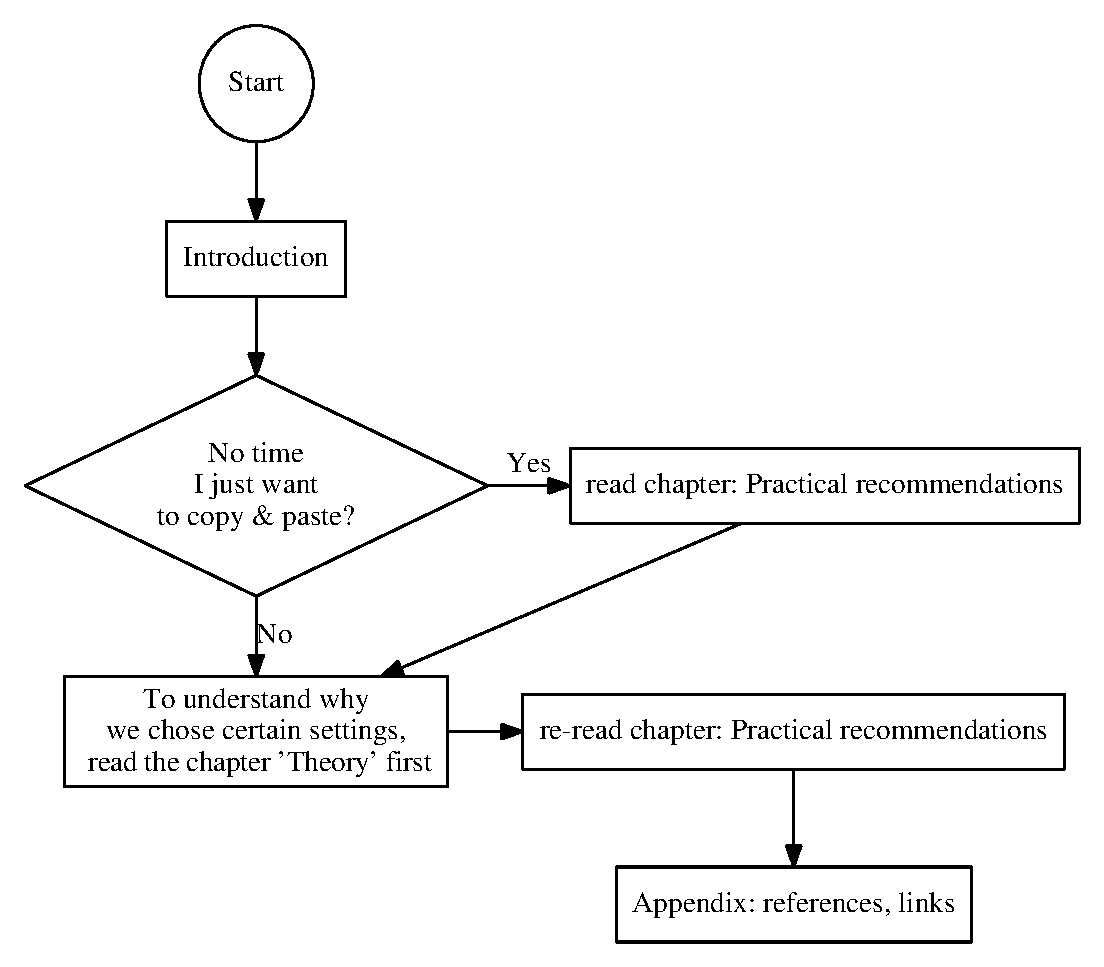
\includegraphics[width=0.65\textwidth]{img/howtoread}
  %\caption{Screenshot of \url{http://www.keylength.com} for 128 bit symmetric key size equivalents}
  \label{fig:howtoread}
\end{figure}

\vskip 2em




\section{Disclaimer and scope}
\label{section:disclaimer}
\label{sec:disclaimer-scope}

\epigraph{``A chain is no stronger than its weakest link, and life is after all a chain''}{William James}
\epigraph{``Encryption works. Properly implemented strong crypto systems are
one of the few things that you can rely on. Unfortunately, endpoint security is
so terrifically weak that NSA can frequently find ways around it.''}{Edward
Snowden, answering questions live on the Guardian's
website~\cite{snowdenGuardianGreenwald}}


This guide specifically does not address physical security, protecting software
and hardware against exploits, basic IT security housekeeping, information
assurance techniques, traffic analysis attacks, issues with key-roll over and
key management, securing client PCs and mobile devices (theft, loss), proper
Operations Security\footnote{\url{https://en.wikipedia.org/wiki/Operations_security}}, social
engineering attacks, protection against tempest~\cite{Wikipedia:Tempest} attack techniques,
thwarting different side-channel attacks (timing--, cache timing--,
differential fault analysis, differential power analysis or power monitoring
attacks), downgrade attacks, jamming the encrypted channel or other similar
attacks which are typically employed to circumvent strong encryption.  The
authors can not overstate the importance of these other techniques.  Interested
readers are advised to read about these attacks in detail since they give a lot
of insight into other parts of cryptography engineering which need to be dealt
with.\footnote{An easy to read yet very insightful recent example is the
"FLUSH+RELOAD" technique~\cite{yarom2013flush+} for leaking cryptographic keys
from one virtual machine to another via L3 cache timing attacks.}

This guide does not talk much about the well-known insecurities of trusting a
public-key infrastructure (PKI)\footnote{Interested readers are referred to
\url{https://bugzilla.mozilla.org/show_bug.cgi?id=647959} or
\url{http://www.h-online.com/security/news/item/Honest-Achmed-asks-for-trust-1231314.html}
which brings the problem of trusting PKIs right to the point}. Nor
does this text fully explain how to run your own Certificate Authority (CA). 


Most of this zoo of information security issues are addressed in the very
comprehensive book ``Security Engineering'' by Ross Anderson~\cite{anderson2008security}. 

For some experts in cryptography this text might seem too informal. However, we
strive to keep the language as non-technical as possible and fitting for our
target audience: system administrators who can collectively improve the
security level for all of their users. 



\epigraph{``Security is a process, not a product.''}{Bruce Schneier}

This guide can only describe what the authors currently
\emph{believe} to be the best settings based on their personal experience and
after intensive cross checking with literature and experts. For a complete list
of people who reviewed this paper, see the \nameref{section:Reviewers}.
Even though multiple specialists reviewed the guide, the authors can give
\emph{no guarantee whatsoever} that they made the right recommendations. Keep in
mind that tomorrow there might be new attacks on some ciphers and many of the
recommendations in this guide might turn out to be wrong. Security is a
process.


We therefore recommend that system administrators keep up to date with recent
topics in IT security and cryptography. 


In this sense, this guide is very focused on getting the cipher strings done
right even though there is much more to do in order to make a system more
secure.  We the authors, need this document as much as the reader needs it.

\subsection*{Scope}
\label{section:Scope}

In this guide, we restricted ourselves to:
\begin{itemize*}
  \item Internet-facing services
  \item Commonly used services
  \item Devices which are used in business environments (this specifically excludes XBoxes, Playstations and similar consumer devices)
  \item OpenSSL 
\end{itemize*}

We explicitly excluded:
\begin{itemize*}
  \item Specialized systems (such as medical devices, most embedded systems, industrial control systems, etc.)
  \item Wireless Access Points
  \item Smart-cards/chip cards
%  \item Advice on running a PKI or a CA
%  \item Services which should be run only in an internal network and never face the Internet.
\end{itemize*}


%%% Local Variables: 
%%% mode: latex
%%% TeX-master: "applied-crypto-hardening"
%%% End: 

%\section{Motivation}
%\label{section:Motivation}

\section{Methods}
\label{section:Methods}

\epigraph{``C.O.S.H.E.R - completely open source, headers, engineering and research}{A. Kaplan's mail signature for many years}
% proof: http://www.mavetju.org/mail/view_message.php?list=freebsd-current&id=947899&raw=yes


For writing this guide, we chose to collect the most well researched facts
about cryptography settings and let as many trusted specialists as possible
review those settings.  The review process is completely open and done on a
public mailing list. The document is available (read-only) to the public
Internet on a git server, GitHub (mirror) and open for public scrutiny.
However, write permissions to the document are only granted to vetted people.
The list of reviewers can be found in the \nameref{section:Reviewers}.  Every
write operation to the document is logged via the ``git'' version control
system and can thus be traced to a specific author.  We accept ``git pull
requests'' on the github
mirror\footnote{\url{https://github.com/BetterCrypto/Applied-Crypto-Hardening}}
for this paper.


\vskip 0.5em

Public peer-review and ``multiple eyes'' checking of our publication is the
best strategy we can imagine at the present moment
\footnote{\url{http://www.wired.com/opinion/2013/10/how-to-design-and-defend-against-the-perfect-backdoor/}}.

\vskip 0.5em
We invite the gentle reader to participate in this public review process.


\section{Scope}
\label{section:Scope}

We restricted ourselves to:
\begin{itemize}
\item Internet-facing services
\item Commonly used services
\item Devices which are used in business environments (this mostly excludes XBoxes, Playstations and similar common consumer devices)
\end{itemize}

We explicitly excluded:
\begin{itemize}
\item Specialized systems (such as medical devices, most embedded systems, etc.)
\item Wireless Access Points
%\item Services which should be run only in an internal network and never face the Internet.
\end{itemize}

%% * whatsapp --> man kann nichts machen, out of scope
%* Lync: == SIP von M$.
%* Skype: man kann ncihts machen, out of scope.
%* Wi-Fi APs, 802.1X, ... ???? --> out of scope
%* Tomcats/...????
%* SIP   -> Klaus???
%* SRTP  -> Klaus???
%* DNSSec ?? Verweis auf BCPxxx  --> out of scope
%   - DANE
%What happens at the IETF at the moment?
%* TOR?? --> out of scope
%* S/Mime --> nachsehen, gibt es BCPs? (--> Ramin)
%* TrueCrypt, LUKS, FileVault, etc ---> out of scope
%* AFS -> out of scope
%* Kerberos --> out of scope
%* NNTP -> out of scope
%* NTPs tlsdate -> out of scope
%* BGP / OSPF --> out of scope
%* irc,silc --> out of scope
%* LDAP -> out of scope
%* Moxa , APC, und co... ICS . Ethernet to serial --> out of scope
%* telnet -> DON't!!!
%* rsyslog --> out of scope
%* ARP bei v6 spoofing -> out of scope
%* tinc?? -> out of scope
%* rsync -> nur ueber ssh fahren ausser public web mirrors
%* telnets -> out of scope
%* ftps -> out of scope
%seclayer-tcp    3495/udp    # securitylayer over tcp
%seclayer-tcp    3495/tcp    # securitylayer over tcp
%* webmin -> maybe
%* plesk -> out of scope
%* phpmyadmin --> haengt am apache, out of scope
%* DSL modems -> out of scope
%* UPnP, natPmp --> out of scope 

\section{Public Key Infrastructures}
\label{section:PKIs}

Public-Key Infrastructures aim to provide a way to simplify the verification of
a certificate's trustworthiness.  For this, certificate authorities (CAs) are
used for creating a signature chain from the CA down to the server (or client).
Accepting a CA as a generally-trusted mediator solves the trust-scaling problem
at the cost of introducing an actor that magically is more trustworthy.

This section deals with settings related to trusting CAs.  However, our main
recommendations for PKIs is: if you are able to run your own PKI and disable
any other CA, do so.  This is mostly possible in any machine 2 machine
communication system where compatibility with external entities is not an issue.

A good background on PKIs can be found in \todo{insert reference}.

\todo{ts: Background and Configuration (EMET) of Certificate Pinning, TLSA integration, 
  When to use self-signed certificates, how to get certificates from public CA authorities 
  (CAcert, StartSSL), Best-practices how to create a CA and how to generate private keys/CSRs, 
  Discussion about OCSP and CRLs. TD: Useful Firefox plugins: CipherFox, Conspiracy, Perspectives.}


%``Certification
%Policy''\footnote{\url{http://en.wikipedia.org/wiki/Certificate_Policy}}
%(CA)

\section{A note on Elliptic Curve Cryptography}
\label{section:EllipticCurveCryptography}

Elliptic Curve Cryptogaphy (simply called ECC from now on) is a branch of 
cryptography that emerged in the mid-1980ties.
The security of the RSA algorithm is based on the assumption that factoring 
large primes is infeasible. Likewise the security of ECC, DH and DSA is 
based on the discrete logrithm problem.
\footnote{\url{http://www.mccurley.org/papers/dlog.pdf}} 
\footnote{\url{http://en.wikipedia.org/wiki/Discrete\_logarithm}}
\footnote{\url{http://mathworld.wolfram.com/EllipticCurve.html}}.
Finding the discrete logarithm of an elliptic curve from its public base
point is thought to be infeasible. This is known as the Elliptic Curve Discrete 
Logarithm Problem (ECDLP). ECC and the underlying mathematical foundation are not easy 
to understand - luckily there have been some great introductions on the topic lately
\footnote{\url{http://arstechnica.com/security/2013/10/a-relatively-easy-to-understand-primer-on-elliptic-curve-cryptography}}
\footnote{\url{https://www.imperialviolet.org/2010/12/04/ecc.html}}
\footnote{\url{http://www.isg.rhul.ac.uk/~sdg/ecc.html}}.

ECC provides for much stronger security with less computonally expensive
operations in comparison to traditional PKI algorithms (See the Section \ref{section:keylengths}).


The security of ECC relies on the elliptic curves and curve points chosen
as parameters for the algorithm in question. Well before the NSA-leak scandal
there has been a lot of discussion regarding these parameters and their 
potential subversion. A part of the discussion involved recommended sets 
of curves and curve points chosen by different standardization bodies such 
as the National Institute of Standards and Technology (NIST) 
\footnote{\url{http://www.nist.gov}}. Which were later widely implemented 
in most common crypto libraries. Those parameters came under question 
repeatedly from cryptographers
\footnote{\url{http://cr.yp.to/talks/2013.09.16/slides-djb-20130916-a4.pdf}}
\footnote{\url{https://www.schneier.com/blog/archives/2013/09/the\_nsa\_is\_brea.html\#c1675929}}
\footnote{\url{http://crypto.stackexchange.com/questions/10263/should-we-trust-the-nist-recommended-ecc-parameters}}.
At the time of writing there is ongoing research as to the security of 
various ECC parameters\cite{DJBSC}.
Most software configured to rely on ECC (be it client or server) is
not able to promote or black-list certain curves. It is the hope of
the authors that such functionality will be deployed widely soon.
The authors of this paper include configurations and recommendations
with and without ECC - the reader may choose to adopt those settings
as he finds best suited to his environment. The authors will not make
this decision for the reader.


\textbf{A word of warning:} One should get familiar with ECC, different curves and
parameters if one chooses to adopt ECC configurations. Since there is much 
discussion on the security of ECC, flawed settings might very well compromise the 
security of the entire system!

%% mention different attacks on ECC besides flawed parameters!


\section{A note on Diffie Hellman Key Exchanges}
\label{section:DH}

\todo{write this. Some thoughts should go into chosing p,g and when the defaults are OK. See also: http://crypto.stackexchange.com/questions/1963/how-large-should-a-diffie-hellman-p-be}

\section{Keylengths}
\label{section:keylengths}


\epigraph{``On the choice between AES256 and AES128: I would never consider
using AES256, just like I don't wear a helmet when I sit inside my car. It's
too much bother for the epsilon improvement in security.''}{-- Vincent Rijmen
in a personal mail exchange Dec 2013}

Recommendations on keylengths need to be adapted regularly. Since this document
first of all is static and second of all, does not consider itself to be
authoritative on keylengths, we would rather refer to existing publications and
websites.  Recommending a safe key length is a hit-and-miss issue.

Furthermore, when chosing an encryption algorithm and keylength, the
designer/sysadmin always needs to consider the value of the information and how
long it must be protected.  In other words: consider the number of years the
data needs to stay confidential.


The ECRYPT II publication (\cite{ii2011ecrypt}) gives a fascinating overview of
strenghts of symmetric keys in chapter 5 and chapter 7. Summarizing ECRYPT II, we
recommend 128 bit of key strenght for symmetric keys. In ECRYPT II, this is
considered safe for security level 7, long term protection.

In the same ECRYPT II publication you can find a practical comparison of key size
equivalence between symmetric key sizes and RSA, discrete log (DLOG) and EC
keylengths. ECRYPT II arrives at the interesting conclusion that for an
equivalence of 128 bit symmetric size, you will need to use an 3248 bit RSA
key. See chapter 7 of \cite{ii2011ecrypt}, page 30.


There are a couple of other studies comparing keylengths and their respective
strengths.  The website \url{http://www.keylength.com/} compares these papers
and offers a good overview of approximations for key lengths based on
recommendations by different standardization bodies and academic publications.
Figure \ref{fig:keylengths.com} shows a typical comparison of keylengths on
this web site.

\begin{figure}[h]
  \centering
  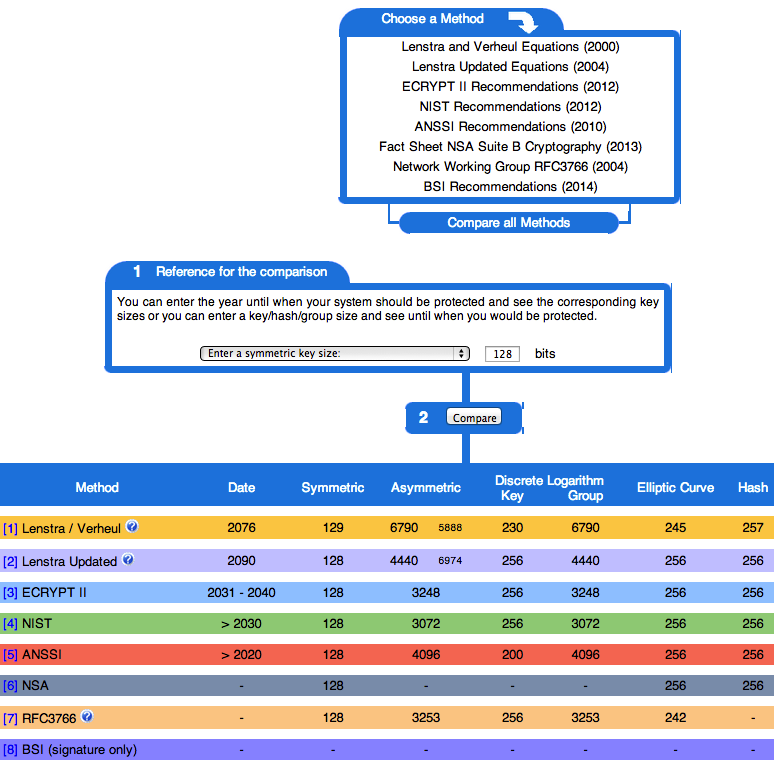
\includegraphics[width=0.65\textwidth]{img/keylengths_com.png}
  \caption{Screenshot of \url{http://www.keylength.com} for 128 bit symmetric key size equivalents}
  \label{fig:keylengths.com}
\end{figure}


\paragraph{Summary}
\begin{itemize}

\item For traditional asymmetric public-key cryptography we consider any key
length below 2048 bits to be deprecated at the time of this writing (for long
term protection).  

\item For elliptic curve cryptography we consider key lengths below 256 bits to
be inadequate for long term protection.  

\item For symmetric algorithms we consider anything below 128 bits to be
inadequate for long term protection.

\end{itemize}

\paragraph{Special remark on 3DES} \mbox{} \\
We want to note that 3DES theoretically has 168 bits of security, however based
on the NIST Special Publication 800-57
\footnote{\url{http://csrc.nist.gov/publications/PubsSPs.html\#800-57-part1},
pages 63 and 64}, it is clear that 3DES can only be considered to provide for
80 bits / 112 bits security.






\section{Random Number Generators}
\label{section:RNGs}

% This section was authored by Ralf Schlatterbeck (Ralf Schlatterbeck <rsc@runtux.com>)

\epigraph{``The generation of random numbers is too important to be left to chance.''}{-- Robert R. Coveyou}


\begin{figure}[h]
  \centering
  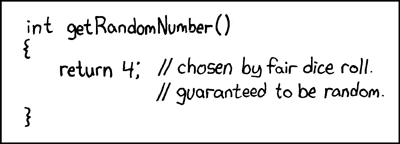
\includegraphics[width=0.4\textwidth]{img/random_number.png}
  \caption{xkcd, source: \url{http://imgs.xkcd.com/comics/random_number.png}, license: CC-BY-NC}
  \label{fig:dilbertRNG}
\end{figure}



A good source of random numbers is essential for many crypto
operations. The key feature of a good random number generator is the
non-predictability of the generated numbers. This means that hardware
support for generating entropy is essential.


Hardware random number generators in operating systems or standalone
components collect entropy from various random events mostly by using
the (low bits of the) time an event occurs as an entropy source. The
entropy is merged into an entropy pool and in some implementations there
is some bookkeeping about the number of random bits available.

\subsection{When random number generators fail}

Random number generators can fail -- returning predictable non-random
numbers -- if not enough entropy is available when random numbers should
be generated.

This typically occurs for embedded devices and virtual machines.
Embedded devices lack some entropy sources other devices have, e.g.:

\begin{itemize}
\item No persistent clock, so boot-time is not contributing to the
    initial RNG state
\item No hard-disk: No entropy from hard-disk timing, no way to store
    entropy between reboots
\end{itemize}

Virtual machines emulate some hardware components so that the
generated entropy is over-estimated. The most critical component that
has been shown to return wrong results in an emulated environment is the
timing source\cite{Eng11,POL11}.

Typically the most vulnerable time where low-entropy situations occur is
shortly after a reboot. Unfortunately many operating system installers
create cryptographic keys shortly after a reboot\cite{HDWH12}.

Another problem is that OpenSSL seeds its internal random generator only
seldomly from the hardware random number generator of the operating
system. This can lead to situations where a daemon that is started at a
time when entropy is low keeps this low-entropy situation for hours
leading to predictable session keys\cite{HDWH12}.

\subsection{Linux}

\todo{Other architectures, BSD, Windows?}

On Linux there are two devices that return random bytes when read, the
\verb+/dev/random+ can block until sufficient entropy has been collected
while \verb+/dev/urandom+ will not block and return whatever (possibly
insufficient) entropy has been collected so far.

Unfortunately most crypto implementations are using \verb+/dev/urandom+
and can produce predictable random numbers if not enough entropy has
been collected\cite{HDWH12}.

Linux supports the injection of additional entropy into the entropy pool
via the device \verb+/dev/random+. On the one hand this is used for
keeping entropy across reboots by storing output of /dev/random into a
file before shutdown and re-injecting the contents during the boot
process. On the other hand this can be used for running a secondary
entropy collector to inject entropy into the kernel entropy pool.

%% specifics for libraries
%% Openssl uses /dev/urandom. See the paper: https://factorable.net/weakkeys12.conference.pdf (section 5.2)
%% What about other libs? 
%% What about other OSes? 


\subsection{Recommendations}

To avoid situations where a newly deployed server hasn't enough
entropy it is recommended to generate keys (e.g. for SSL or SSH) on
a system with enough entropy available and transfer the generated keys
to the server.  This is especially advisable for small embedded devices
or virtual machines.

For embedded devices and virtual machines deploying additional userspace
software that generates entropy and feeds this to kernel entropy pool
(e.g. by writing to \verb+/dev/random+ on Linux) is recommended. Note
that only a process run as root can update the entropy counters in the
kernel, each non-root user-process can feed entropy to the pool but
cannot update the counters\cite{Wikipedia:/dev/random}.

For Linux the \verb+haveged+
implementation\cite{HAV13a} based on the HAVEGE\cite{SS03}
strong random number generator currently looks like the best choice. It
can feed its generated entropy into the kernel entropy pool and recently
has grown a mechanism to monitor the quality of generated random
numbers\cite{HAV13b}. The memory footprint may be too high for small
embedded devices, though.

For systems where -- during the lifetime of the keys -- it is expected
that low-entropy situations occur, RSA keys should be preferred over DSA
keys: For DSA, if there is ever insufficient entropy at the time keys
are used for signing this may lead to repeated ephemeral keys. An
attacker who can guess an ephemeral private key used in such a signature
can compromise the DSA secret key.
For RSA this can lead to discovery of encrypted plaintext or forged
signatures but not to the compromise of the secret key\cite{HDWH12}.

\section{Cipher suites}

Cipher suites are a combination of algorithms to provide for 
Confidentiality, Integrity and Authenticity
\footnote{\url{http://en.wikipedia.org/wiki/Information\_security}} of 
communication. For example: sending encrypted data over the wire does not 
ensure that the data can not be modified (message integrity), similarly
encrypted data can be sent from an adversary. It is therefore paramount to
prove that data has been sent from the desired source (message authenticity).
This concept is known as authenticated encryption
\footnote{\url{http://en.wikipedia.org/wiki/Authenticated\_encryption}}
\footnote{\url{http://www.cs.jhu.edu/~astubble/dss/ae.pdf}}.

\subsection{Forward Secrecy}
Forward Secrecy or Perfect Forward Secrecy is a property of a cipher suite 
that ensures confidentiality even if the server key has been compromised.
Thus if traffic has been recorded it can not be decrypted even if an adversary
has got hold of the decryption key
\footnote{\url{http://en.wikipedia.org/wiki/Forward\_secrecy}}
\footnote{\url{https://www.eff.org/deeplinks/2013/08/pushing-perfect-forward-secrecy-important-web-privacy-protection}}. 

\subsection{Recommended cipher suites}

In principle, system administrators who want to improve their servers need to
make a hard decision between locking out some users while keeping very high
cipher suite security levels or supporting as many users as possible while
lowering some settings. \url{https://www.ssllabs.com/} gives administrators a
tool to test out different settings. The authors used ssllabs.com to arrive at
a set of cipher suites which we will recommend throught this document.
\textbf{Caution: these settings can only represent a subjective choice of the
authors at the time of this writing. It might be a wise choice to select your
own cipher suites based on the instructions in section
\ref{section:ChosingYourOwnCipherSuites}}.


\subsubsection{Configuration A: strong ciphers, fewer clients}

At the time of this writing, we recommend the following set of strong cipher
suites which may be useful in an environment where you do not depend on many,
diverse external clients and where compatibility is not an issue.  An example
of such an environment might be machine 2 machine communications or corporate
environments where you can define the software which must be used.


We arrived at this set of cipher suites by selecting

\begin{itemize}
\item TLS 1.2
\item Perfect forward secrecy / ephemeral Diffie Hellman
\item strong Hashes (SHA-2)
\item GCM as chaining mode if possible 
\end{itemize}

This results in the string:

\begin{lstlisting}[breaklines]
'EECDH+aRSA+AES256:EDH+aRSA+AES256:!SSLv3'
\end{lstlisting}

%$\implies$ resolves to 
%
%\begin{verbatim}
%openssl ciphers -V $string
%\end{verbatim}



\begin{center}

\begin{tabular}{lllllll}
\toprule
\textbf{ID}   & \textbf{OpenSSL Name}       & \textbf{Version} & \textbf{KeyEx} & \textbf{Auth} & \textbf{Cipher} & \textbf{Hash}\\\cmidrule(lr){1-7}
\verb|0xC030| & ECDHE-RSA-AES256-GCM-SHA384 & TLSv1.2          & ECDH           &  RSA          & AESGCM(256)     & AEAD         \\
\verb|0xC028| & ECDHE-RSA-AES256-SHA384     & TLSv1.2          & ECDH           &  RSA          & AES(256)        & SHA384       \\
\verb|0x009F| & DHE-RSA-AES256-GCM-SHA384   & TLSv1.2          & DH             &  RSA          & AESGCM(256)     & AEAD         \\
\verb|0x006B| & DHE-RSA-AES256-SHA256       & TLSv1.2          & DH             &  RSA          & AES(256)        & SHA256       \\
\bottomrule
\end{tabular}
\end{center}


\textbf{Compatibility}

Only clients which support TLS1.2 are covered by these cipher suites (Chrome 30,
Win 7 and Win 8.1 crypto stack, Opera 17, OpenSSL $\ge$ 1.0.1e, Safari 6 / iOS
6.0.1, Safari 7 / OS X 10.9).



\subsubsection{Configuration B: weaker ciphers, many clients}

In this section we propose a slighly "weaker" set of cipher suites. There are
some known weaknesses of for example SHA-1 which is included in this set.
However, the advantage of this set of cipher suites is its wider compatibility
with clients. 


\textbf{In the following document, all further examples in this paper will use Configuration B}.


We arrived at this set of cipher suites by selecting

\begin{itemize}
\item TLS 1.2, TLS 1.1, TLS 1.0
\item allowing SHA-1
\todo{AK: Note that SHA1 is considered broken but if we are in DHE, we might get around it as long as you can not calculate a SHA1 collision ``live'' on the wire}

\end{itemize}

This results in the string:

\begin{lstlisting}[breaklines]
'EECDH+aRSA+AESGCM:EECDH+aRSA+SHA384:EECDH+aRSA+SHA256:EDH+CAMELLIA256:EECDH:EDH+aRSA:+SSLv3:!aNULL:!eNULL:!LOW:!3DES:!MD5:!EXP:!PSK:!SRP:!DSS:!RC4:!SEED:!AES128:!CAMELLIA128:!ECDSA:AES256-SHA'
\end{lstlisting}



\begin{center}
\begin{tabular}{lllllll}
\toprule
\textbf{ID}   & \textbf{OpenSSL Name}       & \textbf{Version} & \textbf{KeyEx} & \textbf{Auth} & \textbf{Cipher} & \textbf{Hash}\\\cmidrule(lr){1-7}
\verb|0xC030| & ECDHE-RSA-AES256-GCM-SHA384 & TLSv1.2          & ECDH           &  RSA          & AESGCM(256)     & AEAD         \\ 
\verb|0xC028| & ECDHE-RSA-AES256-SHA384     & TLSv1.2          & ECDH           &  RSA          & AES(256)        & SHA384       \\ 
\verb|0x009F| & DHE-RSA-AES256-GCM-SHA384   & TLSv1.2          & DH             &  RSA          & AESGCM(256)     & AEAD         \\ 
\verb|0x006B| & DHE-RSA-AES256-SHA256       & TLSv1.2          & DH             &  RSA          & AES(256)        & SHA256       \\ 
\verb|0x0088| & DHE-RSA-CAMELLIA256-SHA     & SSLv3            & DH             &  RSA          & Camellia(256)   & SHA1         \\ 
\verb|0xC014| & ECDHE-RSA-AES256-SHA        & SSLv3            & ECDH           &  RSA          & AES(256)        & SHA1         \\ 
\verb|0x0039| & DHE-RSA-AES256-SHA          & SSLv3            & DH             &  RSA          & AES(256)        & SHA1         \\ 
\verb|0x0035| & AES256-SHA                  & SSLv3            & RSA            &  RSA          & AES(256)        & SHA1         \\
\bottomrule
\end{tabular}
\end{center}

\textbf{Compatibility}

Note that these cipher suites will not work with anything using Windows XP's
crypto stack (IE, Outlook), Java 6, Java 7 and Android 2.3. Java 7 could be
made compatible by installing the "Java Cryptography Extension (JCE) Unlimited
Strength Jurisdiction Policy Files"
(JCE) \footnote{\url{http://www.oracle.com/technetwork/java/javase/downloads/jce-7-download-432124.html}}.
We could not verify yet if installing JCE also fixes the Java 7
DH-parameter length limitation (1024 bit). 

\textbf{Explanation}

For a detailed explanation of the cipher suites chosen, please see
\ref{section:ChoosingYourOwnCipherSuites}. In short, finding the perfect cipher
string is impossible and must be a tradeoff. On the one hand
there are mandatory and optional ciphers defined in a few RFCs, on the other hand
there are clients and servers only implementing subsets of the specification.

Straight forward, we wanted strong ciphers, forward secrecy
\footnote{\url{http://nmav.gnutls.org/2011/12/price-to-pay-for-perfect-forward.html}}
and the most clients we could get while still having a cipher string that can be
used on older servers too (think OpenSSL 0.9.8). This cipher string is meant to be used
by copy and paste and needs to just work.

\begin{itemize}
\item TLS1.2 is preferred over TLSv1.0/SSLv3 (while still providing a useable cipher
      string for SSLv3).
\item AES256 and CAMELLIA256 count as strong ciphers at the moment; preferrably in
      GCM mode.\\
	  \todo{add a reference here please}
      \todo{Adi: add 128bit ciphers too} \\
      \todo{Team: discuss ordering of keys (256 $\rightarrow$ 128 or vice versa?)}
\item DHE or ECDHE for forward secrecy
\item RSA as this will fit most of todays setup
\item AES256-SHA as a last ressort (with this cipher at the end, even systems with
      very old versions of openssl like 0.9.8 will just work. Just forward secrecy
      will not be used. On systems that do not support elliptic curves, that cipher
      offers support for the Microsoft crypto libraries that only support ECDHE.
\end{itemize}
\todo{Adi: review "justification" when next section is written}



\subsection{Known insecure and weak cipher suites}
\todo{PG: please write this section. List all known broken, obsolete, weak and insecure cipher suites . Or even better: find the best site which keeps track of outdated cipher suites and simply reference it. We do not want to maintain such a list ourselves!}

\subsection{Compatibility}
\todo{write this section. The idea here is to first document which server (and openssl) version we assumed. Once these parameters are fixed, we then list all clients which are supported for Variant A) and B). Therefore we can document compatibilities to some extent. The sysadmin can then choose roughly what he looses or gains by omitting certain cipher suites.}


\subsection{Choosing your own cipher suites}
\label{section:ChoosingYourOwnCipherSuites}

\todo{ Adi...  you want to describe how to make your own selection of cipher suites here.}

SSL/TLS cipher suites consist of a key exchange mechanism, an authentication, a
stream cipher (or a block cipher with a chaining mode) and a message authentication
mechanism.

Many of those mechanisms are interchangeable like the key exchange in this example:
\texttt{ECDHE-RSA-AES256-GCM-SHA384} and \texttt{DHE-RSA-AES256-GCM-SHA384}.
To provide a decent level of security, all algorithms need to be safe (subject to
the disclaimer in section \ref{section:disclaimer}).

Note: There are some very weak cipher suites in about every crypto library, most of
them for historic reasons like the crypto export embargo
\footnote{\url{http://en.wikipedia.org/wiki/Export_of_cryptography_in_the_United_States}}.
For the following chapter support of those is assumed to be disabled by having
\texttt{!EXP:!LOW:!NULL} as part of the cipher string.

\todo{Team: do we need references for all cipher suites considered weak?}

\subsubsection{key exchange}

Many algorithms allow a secure key exchange. Among those are RSA, DSA, DH, EDH, ECDSA,
ECDH, EECDH and a few others. During the key exchange, keys for authentication and for
encryption are exchanged. For RSA and DSA those keys are the same.

\begin{center}
\begin{tabular}{| l | l | l | l |}
    \toprule
 & \textbf{Key}  & \textbf{\cellcolor{orange}EC}  & \textbf{\cellcolor{green}ephemeral} \\ \cmidrule(lr){1-4}
    \cellcolor{red}    RSA   & RSA  & \cellcolor{green}no   & \cellcolor{red} no         \\
    \cellcolor{red}    DH    & RSA  & \cellcolor{green}no   & \cellcolor{red} no         \\
    \cellcolor{green}  EDH   & RSA  & \cellcolor{green}no   & \cellcolor{green} yes      \\
    \cellcolor{red}    ECDH  & both & \cellcolor{orange}yes & \cellcolor{red} no         \\
    \cellcolor{orange} EECDH & both & \cellcolor{orange}yes & \cellcolor{green} yes      \\
    \cellcolor{red}    DSA   & DSA  & \cellcolor{green}no   & \cellcolor{red} no         \\
    \cellcolor{red}    ECDSA & DSA  & \cellcolor{orange}yes & \cellcolor{red} no         \\
\bottomrule
\end{tabular}
%\\
%\\
%disabled: \texttt{!PSK:!SRP}
\end{center}

\textbf{Ephemeral Key Exchange} uses different keys for authentication (the server's RSA
key) and encryption (a randomly created key). This advantage is called ``Forward
Secrecy'' and means that even recorded traffic cannot be decrypted later when someone
gets the server key. \\
All ephemeral key exchange mechanisms base on Diffie-Hellman algorithm and require
pre-generated Diffe-Hellman parameter (which allow fast ephemeral key generation). It
is important to note that the Diffie-Hellman parameters need to be at least as strong
(speaking in number of bits) as the RSA host key. %TODO: reference!


\textbf{Elliptic Curves}\ref{section:EllipticCurveCryptography} required by current TLS
standards only consist of the so-called NIST-curves (\texttt{secp256r1} and
\texttt{secp384r1}) which may be weak because the parameters that led to their generation
weren't properly explained (by the NSA). \\
Disabling support for Elliptic Curves leads to no ephemeral key exchange being available
for the Windows platform. When you decide to use Elliptic Curves despite the uncertainty,
make sure to at least use the stronger curve of the two supported by all clients
(\texttt{secp384r1}).


Other key exchange mechanisms like Pre-Shared Key (PSK) or Secure Remote Password
(SRP) are irrelevant for regular SSL/TLS use.

\subsubsection{authentication}

RSA, DSA, DSS, ECDSA, ECDH, FORTEZZA(?).

Other authentication mechanisms like Pre Shared Keys aren't used in SSL/TLS: \texttt{!PSK:!aNULL}

\subsubsection{encryption}

AES, CAMELLIA, SEED, ARIA(?), FORTEZZA(?)...

Other ciphers like IDEA, RC2, RC4, 3DES or DES are weak and therefor not recommended:
\texttt{!DES:!3DES:!RC2:!RC4:!eNULL}

\subsubsection{message authentication}

SHA-1 (SHA), SHA-2 (SHA256, SHA384), AEAD

Note that SHA-1 is considered broken and should not be used. SHA-1 is however a the
only still available message authentication mechanism supporting TLS1.0/SSLv3. Without
SHA-1 most clients will be locked out.

Other hash functions like MD2, MD4 or MD5 are unsafe and broken: \texttt{!MD2:!MD4:!MD5}

\subsubsection{combining cipher strings}
%% reference 'man ciphers' and 'openssl ciphers' and show some simple examples
%% VERY IMPORTANT: hint at the IANA-list and the differences in implementations

\todo{ Adi...  The text below was simply the old text, still left here for reference.}

%%% NOTE: we do not need to list this all here, can move to an appendix
%At the time of this writing, SSL is defined in RFCs: 	
%
%\begin{itemize}
%\item RFC2246 - TLS1.0		
%\item RFC3268 - AES		
%\item RFC4132 - Camelia		
%\item RFC4162 - SEED		
%\item RFC4279 - PSK		
%\item RFC4346 - TLS 1.1		
%\item RFC4492 - ECC		
%\item RFC4785 - PSK\_NULL		
%\item RFC5246 - TLS 1.2		
%\item RFC5288 - AES\_GCM		
%\item RFC5289 - AES\_GCM\_SHA2\_ECC		
%\item RFC5430 - Suite B		
%\item RFC5487 - GCM\_PSK		
%\item RFC5489 - ECDHE\_PSK		
%\item RFC5932 - Camelia		
%\item RFC6101 - SSL 3.0		
%\item RFC6209 - ARIA		
%\item RFC6367 - Camelia		
%\item RFC6655 - AES\_CCM		
%\item RFC7027 - Brainpool Curves		
%\end{itemize}

\subsubsection{Overview of SSL Server settings}


Most Server software (Webservers, Mail servers, etc.) can be configured to prefer certain cipher suites over others. 
We followed the recommendations by Ivan Ristic's SSL/TLS Deployment Best Practices\footnote{\url{https://www.ssllabs.com/projects/best-practices/index.html}} document (see section 2.2 "Use Secure Protocols") and arrived at a list of recommended cipher suites for SSL enabled servers.

Following Ivan Ristic's adivce we arrived at a categorisation of cipher suites.

\begin{center}
\begin{tabular}{lllll}
\cmidrule[\heavyrulewidth]{2-5}
& \textbf{Version}   & \textbf{KeyEx} & \textbf{Cipher}    & \textbf{MAC}       \\\cmidrule(lr){2-5}
\cellcolor{green}prefer  & TLS 1.2   & DHE\_DSS   & AES\_256\_GCM   & SHA384        \\
    &   & DHE\_RSA   & AES\_256\_CCM   & SHA256        \\
    &   & ECDHE\_ECDSA   & AES\_256\_CBC   &       \\
    &   & ECDHE\_RSA &   &       \\ 
    &   &   &   &       \\
\cellcolor{orange}consider    & TLS 1.1   & DH\_DSS    & AES\_128\_GCM   & SHA       \\
    & TLS 1.0   & DH\_RSA    & AES\_128\_CCM   &       \\
    &   & ECDH\_ECDSA    & AES\_128\_CBC   &       \\ 
    &   & ECDH\_RSA  & CAMELLIA\_256\_CBC  &       \\
    &   & RSA   & CAMELLIA\_128\_CBC  &       \\
    &   &   &   &       \\
\cellcolor{red}avoid   
& SSL 3.0   & NULL  & NULL  & NULL      \\
    &   & DH\_anon   & RC4\_128   & MD5       \\
    &   & ECDH\_anon & 3DES\_EDE\_CBC  &       \\
    &   &   & DES\_CBC   &       \\
    &   &   &   &       \\
\cellcolor{blue}{\color{white}special }
&   & PSK   & CAMELLIA\_256\_GCM  &       \\
    &   & DHE\_PSK   & CAMELLIA\_128\_GCM  &       \\
    &   & RSA\_PSK   & ARIA\_256\_GCM  &       \\
    &   & ECDHE\_PSK & ARIA\_256\_CBC  &       \\
    &   &   & ARIA\_128\_GCM  &       \\
    &   &   & ARIA\_128\_CBC  &       \\
    &   &   & SEED  &       \\
\cmidrule[\heavyrulewidth]{2-5}
\end{tabular}
\end{center}

A remark on the ``consider'' section: the BSI (Federal office for information security, Germany) recommends in its technical report TR-02102-2\footnote{\url{https://www.bsi.bund.de/SharedDocs/Downloads/DE/BSI/Publikationen/TechnischeRichtlinien/TR02102/BSI-TR-02102-2_pdf.html}} to \textbf{avoid} non-ephemeral\footnote{Ephemeral keys are session keys which are destroyed upon termination of the encrypted session. In TLS/SSL, they are realized by the DHE cipher suites. } keys for any communication which might contain personal or sensitive data. In this document, we follow BSI's advice and therefore only keep cipher suites containing (EC)DH\textbf{E} (ephemeral) variants. System administrators, who can not use forward secrecy can still use the cipher suites in the ``consider'' section. We however, do not recommend them in this document.

%% NOTE: s/forward secrecy/perfect forward secrecy???

Note that the entries marked as ``special'' are cipher suites which are not common to all clients (webbrowsers etc).


\subsubsection{Tested clients}
 
Next we tested the cipher suites above on the following clients:

%% NOTE: we need to test with more systems!!
\begin{itemize}
\item Chrome 30.0.1599.101 Mac OS X 10.9
\item Safari 7.0 Mac OS X 10.9
\item Firefox 25.0 Mac OS X 10.9
\item Internet Explorer 10 Windows 7
\item Apple iOS 7.0.3
\end{itemize}


The result of testing the cipher suites with these clients gives us a preference order as shown in table \ref{table:prefOrderCipherSuites}. 
Should a client not be able to use a specific cipher suite, it will fall back to the next possible entry as given by the ordering.

\begin{table}[h]
\centering\small
    \begin{tabular}{cllcccc}
    \toprule
    \textbf{Pref}   & \textbf{Cipher Suite}                            & \textbf{ID}   & \multicolumn{4}{l}{\textbf{Supported by}}\\ 
    \cmidrule(lr){4-7}
                    & \textbf{OpenSSL Name}                            &               & Chrome & FF   & IE   & Safari \\
    \cmidrule(lr){1-7}
    \phantom{0}1    & \verb|TLS_DHE_RSA_WITH_AES_256_GCM_SHA384|     & \verb|0x009f| & \no    & \no  & \no  & \no    \\
                    & \verb|DHE-RSA-AES256-GCM-SHA384|                      &               & &&&\\\rowcolor{lightlightgray}
    \phantom{0}2    & \verb|TLS_ECDHE_ECDSA_WITH_AES_256_CBC_SHA384| & \verb|0xC024| & \no    & \no  & \no  & \yes   \\\rowcolor{lightlightgray}
                    & \verb|ECDHE-ECDSA-AES256-SHA384|                      &               & &&&\\
    \phantom{0}3    & \verb|TLS_ECDHE_RSA_WITH_AES_256_CBC_SHA384|   & \verb|0xC028| & \no    & \no  & \no  & \yes   \\
                    & \verb|ECDHE-RSA-AES256-SHA384|                        &               & &&&\\\rowcolor{lightlightgray}
    \phantom{0}4    & \verb|TLS_DHE_RSA_WITH_AES_256_CBC_SHA256|     & \verb|0x006B| & \yes   & \no  & \no  & \yes   \\\rowcolor{lightlightgray}
                    & \verb|DHE-RSA-AES256-SHA256|                          &               & &&&\\
    \phantom{0}5    & \verb|TLS_ECDHE_ECDSA_WITH_AES_256_CBC_SHA|    & \verb|0xC00A| & \yes   & \yes & \yes & \yes   \\
                    & \verb|ECDHE-ECDSA-AES256-SHA|                         &               & &&&\\\rowcolor{lightlightgray}
    \phantom{0}6    & \verb|TLS_ECDHE_RSA_WITH_AES_256_CBC_SHA|      & \verb|0xC014| & \yes   & \yes & \yes & \yes   \\\rowcolor{lightlightgray}
                    & \verb|ECDHE-RSA-AES256-SHA|                           &               & &&&\\
    \phantom{0}7    & \verb|TLS_DHE_RSA_WITH_AES_256_CBC_SHA|        & \verb|0x0039| & \yes   & \yes & \no  & \yes   \\
                    & \verb|DHE-RSA-AES256-SHA|                             &               & &&&\\\rowcolor{lightlightgray}
    \phantom{0}8    & \verb|TLS_DHE_DSS_WITH_AES_256_CBC_SHA|        & \verb|0x0038| & \no    & \yes & \yes & \no    \\\rowcolor{lightlightgray}
                    & \verb|DHE-DSS-AES256-SHA|                             &               & &&&\\
    \phantom{0}9    & \verb|TLS_DHE_RSA_WITH_CAMELLIA_256_CBC_SHA|   & \verb|0x0088| & \no    & \yes & \no  & \no    \\
                    & \verb|DHE-RSA-CAMELLIA256-SHA|                        &               & &&&\\\rowcolor{lightlightgray}
    \phantom{}10    & \verb|TLS_DHE_DSS_WITH_CAMELLIA_256_CBC_SHA|   & \verb|0x0087| & \no    & \yes & \no  & \no    \\\rowcolor{lightlightgray}
                    & \verb|DHE-DSS-CAMELLIA256-SHA|                        &               & &&&\\
   \bottomrule
    \end{tabular}
\caption{Preference order of cipher suites.  All suites are supported by OpenSSL.}
\label{table:prefOrderCipherSuites}
\end{table}

Note: the above table \ref{table:prefOrderCipherSuites} contains Elliptic curve key exchanges. There are currently strong doubts\footnote{\url{http://safecurves.cr.yp.to/rigid.html}} concerning ECC.
If unsure, remove the cipher suites starting with ECDHE in the table above.


Based on this ordering, we can now define the corresponding settings for servers. We will start with the most common web servers.


\section{SSL libraries}
\label{section:ssllibs}

\todo{write down that everything here is very SSL lib dependent. You might have to recompile everythign if you need to change the ssl lib}
\todo{anyone? How about Java? What exists here?}
\todo{Anyone? Windows crypto API?}
\todo{Mac OSX /iOS crypto API? MacLemon?}


\subsection{OpenSSL}

\todo{adi?}

\subsection{GnuTLS}

\todo{adi?}

\subsection{NaCL}

\todo{adi?}

\subsection{polarSSL}

\todo{adi?}

\subsection{matrixSSL}

\todo{adi?}


\newpage
\section{Recommendations on practical settings}
\label{section:PracticalSettings}


\subsection{Webservers}

\subsubsection{Apache}

\begin{description}
\item[Tested with Version:]

\item[Settings:] \mbox{}

%-All +TLSv1.1 +TLSv1.2
\begin{lstlisting}[breaklines]
  SSLProtocol All -SSLv2 -SSLv3 
  SSLHonorCipherOrder On
  SSLCompression off
  # Add six earth month HSTS header for all users...
  Header add Strict-Transport-Security "max-age=15768000"
  # If you want to protect all subdomains, use the following header
  # ALL subdomains HAVE TO support https if you use this!
  # Strict-Transport-Security: max-age=15768000 ; includeSubDomains

  SSLCipherSuite 'EECDH+aRSA+AESGCM:EECDH+aRSA+SHA384:EECDH+aRSA+SHA256:EDH+CAMELLIA256:EECDH:EDH+aRSA:+SSLv3:!aNULL:!eNULL:!LOW:!3DES:!MD5:!EXP:!PSK:!SRP:!DSS:!RC4:!SEED:!AES128:!CAMELLIA128:!ECDSA:AES256-SHA'
\end{lstlisting}

Note again, that any cipher suite starting with ECDHE  can be omitted in case of doubt.
%% XXX NOTE TO SELF: remove from future automatically generated lists!

\item[Additional settings:]

You should redirect everything to httpS:// if possible. In Apache you can do this with the following setting inside of a VirtualHost environment:

\begin{lstlisting}[breaklines]
  <VirtualHost *:80>
   #...
   RewriteEngine On
        RewriteRule ^.*$ https://%{SERVER_NAME}%{REQUEST_URI} [L,R=permanent]
   #...
  </VirtualHost>
\end{lstlisting}

\item[Justification for special settings (if needed):]

\item[References:]

\item[How to test:]

See ssllabs in section \ref{section:Tools}

\end{description}
%XXXX   ECDH+AES256:DH+AES256:ECDH+AES128:DH+AES:ECDH+3DES:DH+3DES:RSA+AES:RSA+3DES:!ADH:!AECDH:!MD5:!DSS


\subsubsection{lighttpd}



\begin{description}
\item[Tested with Version:]

\todo{version?}

\item[Settings:] \mbox{}


%% Complete ssl.cipher-list with same algo than Apache
\todo{FIXME: this string seems to be wrongly formatted??}

\begin{lstlisting}[breaklines]
  $SERVER["socket"] == "0.0.0.0:443" {
    ssl.engine  = "enable"
    ssl.use-sslv2 = "disable"
    ssl.use-sslv3 = "disable"
    #ssl.use-compression obsolete >= 1.4.3.1
    ssl.pemfile = "/etc/lighttpd/server.pem"
    ssl.cipher-list = 'EECDH+aRSA+AESGCM:EECDH+aRSA+SHA384:EECDH+aRSA+SHA256:EDH+CAMELLIA256:EECDH:EDH+aRSA:+SSLv3:!aNULL:!eNULL:!LOW:!3DES:!MD5:!EXP:!PSK:!SRP:!DSS:!RC4:!SEED:!AES128:!CAMELLIA128:!ECDSA:AES256-SHA'
    ssl.honor-cipher-order = "enable"
    setenv.add-response-header  = ( "Strict-Transport-Security" => "max-age=31536000")
  }
\end{lstlisting}


\item[Additional settings:]

As for any other webserver, you should redirect automatically http traffic toward httpS://

\begin{lstlisting}[breaklines]
  $HTTP["scheme"] == "http" {
    # capture vhost name with regex conditiona -> %0 in redirect pattern
    # must be the most inner block to the redirect rule
    $HTTP["host"] =~ ".*" {
        url.redirect = (".*" => "https://%0$0")
    }
  }
\end{lstlisting}


\item[References:] 
\todo{add references}.
lighttpd httpS:// redirection: \url{http://redmine.lighttpd.net/projects/1/wiki/HowToRedirectHttpToHttps}

% add any further references or best practice documents here

\item[How to test:] See ssllabs in section \ref{section:Tools}

% describe here or point the admin to tools (can be a simple footnote or \ref{} to  the tools section) which help the admin to test his settings.
\end{description}


\subsubsection{nginx}

\begin{description}
\item[Tested with Version:]

\todo{version?}

\item[Settings:] \mbox{}

\begin{lstlisting}[breaklines]
  ssl_prefer_server_ciphers on;
  ssl_protocols -SSLv2 -SSLv3; 
  ssl_ciphers 'EECDH+aRSA+AESGCM:EECDH+aRSA+SHA384:EECDH+aRSA+SHA256:EDH+CAMELLIA256:EECDH:EDH+aRSA:+SSLv3:!aNULL:!eNULL:!LOW:!3DES:!MD5:!EXP:!PSK:!SRP:!DSS:!RC4:!SEED:!AES128:!CAMELLIA128:!ECDSA:AES256-SHA';
  add_header Strict-Transport-Security max-age=2592000;
  add_header X-Frame-Options DENY;
\end{lstlisting}

%% XXX FIXME: do we need to specify dhparams? Parameter: ssl_dhparam = file. See: http://wiki.nginx.org/HttpSslModule#ssl_protocols

\item[Additional settings:]

If you decide to trust NIST's ECC curve recommendation, you can add the following line to nginx's configuration file to select special curves:

\begin{lstlisting}[breaklines]
  ssl_ecdh_curve          sect571k1;
\end{lstlisting}

You should redirect everything to httpS:// if possible. In Nginx you can do this with the following setting:

\begin{lstlisting}[breaklines]
  rewrite     ^(.*)   https://$host$1 permanent;
\end{lstlisting}


\item[References:] \todo{add references}

\item[How to test:] See ssllabs in section \ref{section:Tools}

\end{description}





\subsubsection{MS IIS}
\label{sec:ms-iis}


\todo{Daniel: add screenshots and registry keys}

\begin{description}

\item[Tested with Version:] \todo{Daniel: add tested version}

\item[Settings:] \mbox{}


When trying to avoid RC4 and CBC (BEAST-Attack) and requiring perfect
forward secrecy, Microsoft Internet Information Server (IIS) supports
ECDSA, but does not support RSA for key exchange (consider ECC suite
B doubts\footnote{\url{http://safecurves.cr.yp.to/rigid.html}}).

Since \verb|ECDHE_RSA_*| is not supported, a SSL certificate based on
elliptic curves needs to be used.

The configuration of cipher suites MS IIS will use can be configured in one
of the following ways:
\begin{enumerate}
\item Group Policy \footnote{\url{http://msdn.microsoft.com/en-us/library/windows/desktop/bb870930(v=vs.85).aspx}}
\item Registry
\item IIS Crypto~\footnote{\url{https://www.nartac.com/Products/IISCrypto/}}
\end{enumerate}


Table~\ref{tab:MS_IIS_Client_Support} shows the process of turning on
one algorithm after another and the effect on the supported Clients
tested using https://www.ssllabs.com.

\verb|SSL 3.0|, \verb|SSL 2.0| and \verb|MD5| are turned off.
\verb|TLS 1.0| and \verb|TLS 2.0| are turned on.

\begin{table}[h]
  \centering
  \small
  \begin{tabular}{ll}
    \toprule
    Cipher Suite & Client \\
    \midrule
    \verb|TLS_ECDHE_ECDSA_WITH_AES_128_GCM_SHA256| & only IE 10,11, OpenSSL 1.0.1e \\
    \verb|TLS_ECDHE_ECDSA_WITH_AES_128_CBC_SHA256| & Chrome 30, Opera 17, Safari 6+ \\
    \verb|TLS_ECDHE_ECDSA_WITH_AES_128_CBC_SHA| & FF 10-24, IE 8+, Safari 5, Java 7\\
    \bottomrule 
 \end{tabular}
  \caption{Client support}
  \label{tab:MS_IIS_Client_Support}
\end{table}

Table~\ref{tab:MS_IIS_Client_Support} shows the algoriths from
strongest to weakest and why they need to be added in this order. For
example insisting on SHA-2 algorithms (only first two lines) would
eliminate all versions of Firefox, so the last line is needed to
support this browser, but should be placed at the bottom, so capable
browsers will choose the stronger SHA-2 algorithms.

\verb|TLS_RSA_WITH_RC4_128_SHA| or equivalent should also be added if
MS Terminal Server Connection is used (make sure to use this only in a
trusted environment). This suite will not be used for SSL, since we do
not use a RSA Key.


% \verb|TLS_ECDHE_ECDSA_WITH_AES_128_GCM_SHA256| ... only supported by: IE 10,11, OpenSSL 1.0.1e
% \verb|TLS_ECDHE_ECDSA_WITH_AES_128_CBC_SHA256| ... Chrome 30, Opera 17, Safari 6+
% \verb|TLS_ECDHE_ECDSA_WITH_AES_128_CBC_SHA| ... Firefox 10-24, IE 8+, Safari 5, Java 7


Not supported Clients:
\begin{enumerate}
\item Java 6
\item WinXP
\item Bing
\end{enumerate}

\item[Additional settings:]

%Here you can add additional settings

\item[Justification for special settings (if needed):]

% in case you have the need for further justifications why you chose this and that setting or if the settings do not fit into the standard Variant A or Variant B schema, please document this here

\item[References:]

\todo{add references}

% add any further references or best practice documents here

\item[How to test:] See ssllabs in section \ref{section:Tools}


\end{description}



\subsection{Mail Servers}

This section documents the most common mail (SMTP) and IMAPs/POPs servers. Another option to secure IMAPs/POPs servers is to place them behind an stunnel server. 

\subsubsection{Dovecot}


Dovecot 2.2:

% Example: http://dovecot.org/list/dovecot/2013-October/092999.html

\begin{lstlisting}[breaklines]
  ssl_cipher_list = 'EECDH+aRSA+AESGCM:EECDH+aRSA+SHA384:EECDH+aRSA+SHA256:EDH+CAMELLIA256:EECDH:EDH+aRSA:+SSLv3:!aNULL:!eNULL:!LOW:!3DES:!MD5:!EXP:!PSK:!SRP:!DSS:!RC4:!SEED:!AES128:!CAMELLIA128:!ECDSA:AES256-SHA'
  ssl_prefer_server_ciphers = yes
\end{lstlisting}

Dovecot 2.1: Almost as good as dovecot 2.2. Does not support ssl\_prefer\_server\_ciphers

\paragraph*{Limitations}\mbox{}\\

Dovecot currently does not support disabling TLS compression. Furthermore, DH parameters
greater than 1024bit aren't possible. The most recent version 2.2.7 of Dovecot implements
configurable DH parameter length
\footnote{\url{http://hg.dovecot.org/dovecot-2.2/rev/43ab5abeb8f0}}.

\subsubsection{cyrus-imapd (based on 2.4.17)}

\paragraph*{imapd.conf}\mbox{}\\

To activate SSL/TLS configure your certificate with
\begin{lstlisting}[breaklines]
  tls_cert_file: .../cert.pem
  tls_key_file: .../cert.key
\end{lstlisting}

Do not forget to add necessary intermediate certificates to the .pem file.\\

Limiting the ciphers provided may force (especially older) clients to connect without encryption at all! Sticking to the defaults is recommended.\\

If you still want to force strong encryption use
\begin{lstlisting}[breaklines]
  tls_cipher_list: <...recommended ciphersuite...>
\end{lstlisting}

cyrus-imapd loads hardcoded 1024 bit DH parameters using get\_rfc2409\_prime\_1024() by default. If you want to load your own DH parameters add them PEM encoded to the certificate file given in tls\_cert\_file. Do not forget to re-add them after updating your certificate.\\

To prevent unencrypted connections on the STARTTLS ports you can set
\begin{lstlisting}[breaklines]
  allowplaintext: 0
\end{lstlisting}
This way MUAs can only authenticate after STARTTLS if you only provide plaintext and SASL PLAIN login methods. Therefore providing CRAM-MD5 or DIGEST-MD5 methods is not recommended.\\

\paragraph*{cyrus.conf}\mbox{}\\

To support POP3/IMAP on ports 110/143 with STARTTLS add
\begin{lstlisting}[breaklines]
  imap         cmd="imapd" listen="imap" prefork=3
  pop3         cmd="pop3d" listen="pop3" prefork=1
\end{lstlisting}
to the SERVICES section.\\

To support POP3S/IMAPS on ports 995/993 add
\begin{lstlisting}[breaklines]
  imaps        cmd="imapd -s" listen="imaps" prefork=3
  pop3s        cmd="pop3d -s" listen="pop3s" prefork=1
\end{lstlisting}


\paragraph*{Limitations}\mbox{}\\

cyrus-imapd currently (2.4.17, trunk) does not support elliptic curves. ECDHE will not work even if defined in your cipher list.\\

Currently there is no way to prefer server ciphers or to disable compression.\\

There is a working patch for all three features:
\url{https://bugzilla.cyrusimap.org/show_bug.cgi?id=3823}\\





% XXX config von Adi?
% sslVersion = TLSv1
% ciphers = EDH+CAMELLIA256:EDH+aRSA:+SSLv3:!aNULL:!eNULL:!LOW:!3DES:!MD5:!EXP:!PSK:!SRP:!DSS:!RC4:!SEED:-AES128:!CAMELLIA128:!ECDSA:AES256-SHA:EDH+AES128;
% options = CIPHER_SERVER_PREFERENCE
% TIMEOUTclose = 1

\subsubsection{SMTP in general}

SMTP usually uses opportunistic TLS. This means that an MTA will accept TLS connections when asked for it during handshake but will not require it. One should always support incoming opportunistic TLS and always try TLS handshake outgoing.\\

Furthermore a mailserver can operate in three modes:
\begin{itemize}
\item As MSA (Mail Submission Agent) your mailserver receives mail from your clients MUAs (Mail User Agent).
\item As receiving MTA (Mail Transmission Agent, MX)
\item As sending MTA (SMTP client)
\end{itemize}
\mbox{}\\
We recommend the following basic setup for all modes:
\begin{itemize}
\item correctly setup MX, A and PTR RRs without using CNAMEs at all.
\item enable encryption (opportunistic TLS)
\item do not use self signed certificates
\end{itemize}

For SMTP client mode we additionally recommend:
\begin{itemize}
\item the hostname used as HELO must match the PTR RR
\item setup a client certificate (most server certificates are client certificates as well)
\item either the common name or at least an alternate subject name of your certificate must match the PTR RR
\item do not modify the cipher suite for client mode
\end{itemize}

For MSA operation we recommend:
\begin{itemize}
\item listen on submission port 587
\item enforce SMTP AUTH even for local networks
\item do not allow SMTP AUTH on unencrypted connections
\item optionally use the recommended cipher suites if (and only if) all your connecting MUAs support them
\end{itemize}



% Note that (with the exception of MSA mode), it might be better to allow any cipher suite -- since any encryption is better than no encryption when it comes to opportunistic TLS.

We strongly recommend to allow all cipher suites for anything but MSA
mode, because the alternative is plain text transmission.

\subsubsection{Postfix}

\begin{description}
\item[Tested with Version:] \mbox{}

\begin{itemize}
\item Postfix 2.9.6 (Debian Wheezy)
\end{itemize}

\item[Settings:] \mbox{}

First, you need to generate Diffie Hellman parameters (please first take a look at the section \ref{section:PRNG}):

\todo{FIXME: this is a really weak setting! See also: http://postfix.1071664.n5.nabble.com/postfix-hardening-what-can-we-do-td61874.html}
\begin{lstlisting}[breaklines]
  % openssl gendh -out /etc/postfix/dh_param_512.pem -2 512
  % openssl gendh -out /etc/postfix/dh_param_1024.pem -2 1024
\end{lstlisting}

Next, we specify these DH parameters in \verb|main.cf|:

\begin{lstlisting}[breaklines]
  smtpd_tls_dh512_param_file = /etc/postfix/dh_param_512.pem
  smtpd_tls_dh1024_param_file = /etc/postfix/dh_param_1024.pem
\end{lstlisting}

\paragraph*{MX and SMTP client configuration}\mbox{}\\

As discussed above, because of opportunistic encryption we do not
restrict the list of ciphers. There's still some steps needed to
enable TLS, all in \verb|main.cf|:

\begin{lstlisting}[breaklines]
  smtpd_tls_cert_file = /etc/postfix/server.pem
  smtpd_tls_key_file = /etc/postfix/server.key
  # use 0 for Postfix >= 2.9, and 1 for earlier versions
  smtpd_tls_loglevel = 0
  # enable opportunistic TLS support in the SMTP server and client
  smtpd_tls_security_level = may
  smtp_tls_security_level = may
  # if you have authentication enabled, only offer it after STARTTLS
  smtpd_tls_auth_only = yes
  tls_ssl_options=NO_COMPRESSION
  tls_random_source = dev:/dev/urandom		
\end{lstlisting}

\paragraph*{MSA}\mbox{}\\

For the MSA \verb|smtpd| process, we first define the ciphers that are
acceptable for the ``mandatory'' security level, again in
\verb|main.cf|:

\begin{lstlisting}[breaklines]
  smtpd_tls_mandatory_protocols = !SSLv2, !SSLv3
  smtpd_tls_mandatory_ciphers=high
  tls_high_cipherlist=EECDH+aRSA+AESGCM:EECDH+aRSA+SHA384:EECDH+aRSA+SHA256:EDH+CAMELLIA256:EECDH:EDH+aRSA:+SSLv3:!aNULL:!eNULL:!LOW:!3DES:!MD5:!EXP:!PSK:!SRP:!DSS:!RC4:!SEED:!AES128:!CAMELLIA128:!ECDSA:AES256-SHA
\end{lstlisting}

Then, we configure the MSA smtpd in \verb|master.cf| with two
additional options that are only used for this instance of smtpd:

\begin{lstlisting}[breaklines]
587       inet  n       -       -       -       -       smtpd 
        -o smtpd_tls_security_level=encrypt -o tls_preempt_cipherlist = yes
\end{lstlisting}

For those users who want to use ECC key exchange, it is possible to specify this via:
\begin{lstlisting}[breaklines]
  smtpd_tls_eecdh_grade = ultra
\end{lstlisting}

\item[Limitations:] \mbox{}

tls\_ssl\_options is supported from Postfix 2.11 onwards. You can
leave the statement in the configuration for older versions, it will
be ignored.

tls\_preempt\_cipherlist is supported from Postfix 2.8 onwards. Again,
you can leave the statement in for older versions.

\item[References:]

Refer to \url{http://www.postfix.org/TLS_README.html} for an in-depth
discussion.

% \item[Additional settings:]
% no additional settings

% \item[Justification for special settings (if needed):]
% no special settings

\item[How to test:]

You can check the effect of the settings with the following command:
\begin{lstlisting}[breaklines]
$ zegrep "TLS connection established from.*with cipher" | /var/log/mail.log | awk '{printf("%s %s %s %s\n", $12, $13, $14, $15)}' | sort | uniq -c | sort -n
      1 SSLv3 with cipher DHE-RSA-AES256-SHA
     23 TLSv1.2 with cipher DHE-RSA-AES256-GCM-SHA384
     60 TLSv1 with cipher ECDHE-RSA-AES256-SHA
    270 TLSv1.2 with cipher ECDHE-RSA-AES256-GCM-SHA384
    335 TLSv1 with cipher DHE-RSA-AES256-SHA
\end{lstlisting}

\end{description}

\subsubsection{Exim (based on 4.82)}

It is highly recommended to read

\url{http://exim.org/exim-html-current/doc/html/spec_html/ch-encrypted_smtp_connections_using_tlsssl.html}

first.

\paragraph*{MSA mode (submission)}\mbox{}\\

In the main config section of Exim add:

\begin{lstlisting}[breaklines]
  tls_certificate = ..../cert.pem
  tls_privatekey = ..../cert.key
\end{lstlisting}
don't forget to add intermediate certificates to the .pem file if needed.\\
\\
Tell Exim to advertise STARTTLS in the EHLO answer to everyone:
\begin{lstlisting}[breaklines]
  tls_advertise_hosts = *
\end{lstlisting}

If you want to support legacy SMTPS on port 465, and STARTTLS on smtp(25)/submission(587) ports set
\begin{lstlisting}[breaklines]
  daemon_smtp_ports = smtp : smtps : submission
  tls_on_connect_ports = 465
\end{lstlisting}
\mbox{}\\
It is highly recommended to limit SMTP AUTH to SSL connections only. To do so add
\begin{lstlisting}[breaklines]
  server_advertise_condition = ${if eq{$tls_cipher}{}{no}{yes}}
\end{lstlisting}
to every authenticator defined.\\

Add the following rules on top of your acl\_smtp\_mail:
\begin{lstlisting}[breaklines]
  warn    hosts           = *
          control         = submission/sender_retain
\end{lstlisting}
This switches Exim to submission mode and allows addition of missing Message-ID: and Date: headers.\\

It is not advisable to restrict the default cipher list for MSA mode if you don't know all connecting MUAs. If you still want to define one please consult the Exim documentation or ask on the exim-users mailinglist.\\
% Exim maintainers do not recommend to change default ciphers
% I think we shouldn't, too
%use:
%\begin{lstlisting}[breaklines]
%  tls_require_ciphers = <...recommended ciphersuite...>
%\end{lstlisting}

The cipher used is written to the logfiles by default. You may want to add
\begin{lstlisting}[breaklines]
  log_selector = <....whatever your log_selector already contains...> \
   +tls_certificate_verified +tls_peerdn +tls_sni
\end{lstlisting}
to get even more TLS information logged.


\paragraph*{server mode (incoming)}\mbox{}\\

In the main config section of Exim add:

\begin{lstlisting}[breaklines]
  tls_certificate = ..../cert.pem
  tls_privatekey = ..../cert.key
\end{lstlisting}
don't forget to add intermediate certificates to the .pem file if needed.\\
\\
Tell Exim to advertise STARTTLS in the EHLO answer to everyone:
\begin{lstlisting}[breaklines]
  tls_advertise_hosts = *
\end{lstlisting}

Listen on smtp(25) port only
\begin{lstlisting}[breaklines]
  daemon_smtp_ports = smtp
\end{lstlisting}

It is not advisable to restrict the default cipher list for opportunistic encryption as used by SMTP. Do not use cipher lists recommended for HTTPS! If you still want to define one please consult the Exim documentation or ask on the exim-users mailinglist.\\
% Exim maintainers do not recommend to change default ciphers
% We shouldn't, too
%use:
%\begin{lstlisting}[breaklines]
%  tls_require_ciphers = <...recommended ciphersuite...>
%\end{lstlisting}

If you want to request and verify client certificates from sending hosts set
\begin{lstlisting}[breaklines]
  tls_verify_certificates = /etc/pki/tls/certs/ca-bundle.crt
  tls_try_verify_hosts = *
\end{lstlisting}

tls\_try\_verify\_hosts only reports the result to your logfile. If you want to disconnect such clients you have to use
\begin{lstlisting}[breaklines]
  tls_verify_hosts = *
\end{lstlisting}

The cipher used is written to the logfiles by default. You may want to add
\begin{lstlisting}[breaklines]
  log_selector = <....whatever your log_selector already contains...> \
   +tls_certificate_verified +tls_peerdn +tls_sni
\end{lstlisting}
to get even more TLS information logged.

\paragraph*{client mode (outgoing)}\mbox{}\\

Exim uses opportunistic encryption in the SMTP transport by default.

Client mode settings have to be done in the configuration section of the smtp transport (driver = smtp).

If you want to use a client certificate (most server certificates can be used as client certificate, too) set
\begin{lstlisting}[breaklines]
  tls_certificate   = .../cert.pem
  tls_privatekey    = .../cert.key
\end{lstlisting}
This is recommended for MTA-MTA traffic.\\

%If you want to limit used ciphers set
%\begin{lstlisting}[breaklines]
%  tls_require_ciphers = <...recommended ciphersuite...>
%\end{lstlisting}
% Exim Maintainers do not recommend ciphers. We shouldn't do so, too.
Do not limit ciphers without a very good reason. In the worst case you end up without encryption at all instead of some weak encryption. Please consult the Exim documentation if you really need to define ciphers.

\paragraph*{OpenSSL}\mbox{}\\
Exim already disables SSLv2 by default. We recommend to add
\begin{lstlisting}[breaklines]
  openssl_options = +all +no_sslv2 +no_compression +cipher_server_preference
\end{lstlisting}
to the main configuration.\\
Note: +all is misleading here since OpenSSL only activates the most common workarounds. But that's how SSL\_OP\_ALL is defined.\\

You do not need to set dh\_parameters. Exim with OpenSSL by default uses parameter initialization with the "2048-bit MODP Group with 224-bit Prime Order Subgroup" defined in section 2.2 of RFC 5114 (ike23).
If you want to set your own DH parameters please read the TLS documentation of exim.\\



\paragraph*{GnuTLS}\mbox{}\\

GnuTLS is different in only some respects to OpenSSL:
\begin{itemize}
\item tls\_require\_ciphers needs a GnuTLS priority string instead of a cipher list. It is recommended to use the defaults by not defining this option. It highly depends on the version of GnuTLS used. Therefore it is not advisable to change the defaults.
\item There is no option like openssl\_options
\end{itemize}

\paragraph*{Exim string expansion}\mbox{}\\

Note that most of the options accept expansion strings. This way you can eg. set cipher lists or STARTTLS advertisment conditionally. Please follow the link to the official Exim documentation to get more information.

\paragraph*{Limitations}\mbox{}\\

Exim currently (4.82) does not support elliptic curves with OpenSSL. This means that ECDHE is not used even if defined in your cipher list.
There already is a working patch to provide support:\\
\url{http://bugs.exim.org/show_bug.cgi?id=1397}


% do we need to documment starttls in detail?
%\subsubsection{starttls?}

\subsection{OpenSSH}
\paragraph*{sshd_config}
\begin{lstlisting}[breaklines]
	# ...

	Protocol 2
	PermitEmptyPasswords no
	PermitRootLogin no
	StrictModes yes
	HostKey /etc/ssh/ssh_host_rsa_key
	Ciphers aes256-gcm@openssh.com aes128-gcm@openssh.com aes256-ctr aes128-ctr
	MACs umac-128-etm@openssh.com,hmac-sha2-512,hmac-sha2-256,hmac-ripemd160
	KexAlgorithms curve25519-sha256@libssh.org,diffie-hellman-group-exchange-sha256,diffie-hellman-group-exchange-sha1,diffie-hellman-group14-sha1
\end{lstlisting}

% XXX: curve25519-sha256@libssh.org only available upstream(!)
Note: Older linux systems won't support SHA2. PuTTY (Windows) does not support RIPE-MD160. Curve25519, AES-GCM and UMAC are only available upstream (OpenSSH 6.1). DSA host keys have been removed on purpose, the DSS standard does not support for DSA keys stronger than 1024bit
\footnote{\url{https://bugzilla.mindrot.org/show_bug.cgi?id=1647}} 
which is far below current standards (see section \ref{section:keylengths}). Legacy systems can use this configuration and simply omit unsupported ciphers, key exchange algorithms and MACs.
\\


\subsection{VPNs}
\todo{write this subsection}
\subsubsection{IPSec}
\label{section:IPSECgeneral}


\todo{cm: check if there are downgrade attacks for checkpoint \& co} \\

\begin{description}

\item[Settings:] \mbox{}

\paragraph*{Assumptions}\mbox{}\\

We assume the usage of IKE (v1 or v2) for this document, and ESP.

\paragraph*{Authentication}\mbox{}\\

IPSEC authentication should optimally be performed via RSA signatures,
with a key size of 2048 bits or more. Configuring only the trusted CA
that issued the peer certificate provides for additional protection
against fake certificates.

If you need to use Pre-Shared Key authentication:

\begin{enumerate}
\item Choose a \textbf{random}, \textbf{long enough} PSK (see below)
\item Use a \textbf{separate} PSK for any IPSEC connection
\item Change the PSKs regularily
\end{enumerate}

The size of the PSK should not be shorter than the output size of
the hash algorithm used in IKE \footnote{It is used in a HMAC, see
  \url{http://www.ietf.org/rfc/rfc2104.txt}.}.

For a key composed of upper- and lowercase letters, numbers, and two
additional symbols \footnote{64 possible values = 6 bits}, that gives
the following minimum lengths in characters:

\begin{table}[h]
  \centering
  \small
  \begin{tabular}{lc}
    \toprule
    IKE Hash & PSK length \\
    \midrule
    SHA256 & 43 \\
    SHA384 & 64 \\
    SHA512 & 86 \\
    \bottomrule
  \end{tabular}
\end{table}

\paragraph*{Cryptographic Suites}\mbox{}\\

IPSEC Cryptographic Suites are pre-defined settings for all the
items of a configuration; they try to provide a balanced security
level and make setting up VPNs easier.

When using any of those suites, make sure to enable ``Perfect Forward
Secrecy`` for Phase 2, as this is not specified in the suites. The
equivalents to the recommended ciphers suites in section
\ref{section:recommendedciphers} are:

\begin{table}[h]
  \centering
  \small
  \begin{tabular}{lll}
    \toprule
    Configuration A & Configuration B & Notes\\
    \midrule
    \verb|Suite-B-GCM-256|\footnote{\url{http://tools.ietf.org/html/rfc6379}} &
\verb|Suite-B-GCM-128| & Uses NIST elliptic curves
\\ & \verb|VPN-B|\footnote{\url{http://tools.ietf.org/html/rfc4308}} &
\\
    \bottomrule
  \end{tabular}
\end{table}

\paragraph*{IKE or Phase 1}\mbox{}\\

Alternatively to the pre-defined cipher suites, you can define your
own, as described in this and the next section.

IKE or Phase 1 is the mutual authentication and key exchange phase.

Use only ``main mode``, as ``aggressive mode`` has known security
vulnerabilities \footnote{\url{http://ikecrack.sourceforge.net/}}.

\todo{how to make footnotes in a table appear in the output document?}

\begin{table}
  \centering
  \small
  \begin{tabular}{lll}
    \toprule
    & Configuration A & Configuration B \\
    \midrule
    Mode & Main Mode & Main Mode \\
    Encryption & AES-256 & AES-256, CAMELLIA-256 \\
    Hash & SHA2-* & SHA2-*, SHA1 \\
    DH Group & Group 14--18 \footnote{2048--8192 bit DH},
    19--21\footnote{(256--521 bit ECDH)} & Group 14--21 \\
    Lifetime & \todo{need recommendations; 1 day seems to be common
      practice} & \\
    \bottomrule
  \end{tabular}
\end{table}

\paragraph*{ESP or Phase 2}\mbox{}\\

ESP or Phase 2 is where the actual data are protected.

\todo{make the tables appear right here!}

\begin{table}
  \centering
  \small
  \begin{tabular}{lll}
    \toprule
    & Configuration A & Configuration B \\
    \midrule
    Perfect Forward Secrecy & yes & yes \\
    Encryption & AES-GCM-16, AES-CTR, AES-CCM-16, AES-256 & AES-GCM-16, AES-CTR, AES-CCM-16, AES-256, CAMELLIA-256 \\
    Hash & SHA2-* (or none for AES-GCM) & SHA2-*, SHA1 (or none for AES-GCM) \\
    DH Group & Same as Phase 1 & Same as Phase 1 \\
    Lifetime & \todo{need recommendations; 1-8 hours is common} & \\
    \bottomrule
  \end{tabular}
\end{table}

\item[References:] \mbox{}

``A Cryptographic Evaluation of IPsec'', Niels Ferguson and Bruce
  Schneier: \url{https://www.schneier.com/paper-ipsec.pdf}

\end{description}

\subsubsection{Check Point FireWall-1}
   
\begin{description}
\item[Tested with Version:] \mbox{}

\begin{itemize}
\item R77 (should work with any currently supported version)
\end{itemize}

\item[Settings:] \mbox{}

Please see section \ref{section:IPSECgeneral} for guidance on
parameter choice. In this section, we will configure a strong setup
according to ``Configuration A''.

This is based on the concept of a ``VPN Community'', which has all the
settings for the gateways that are included in that community.
Communities can be found in the ``IPSEC VPN'' tab of SmartDashboard.

\todo{make those graphics prettier -- whoever has the right LaTeX
  mojo, please do!}

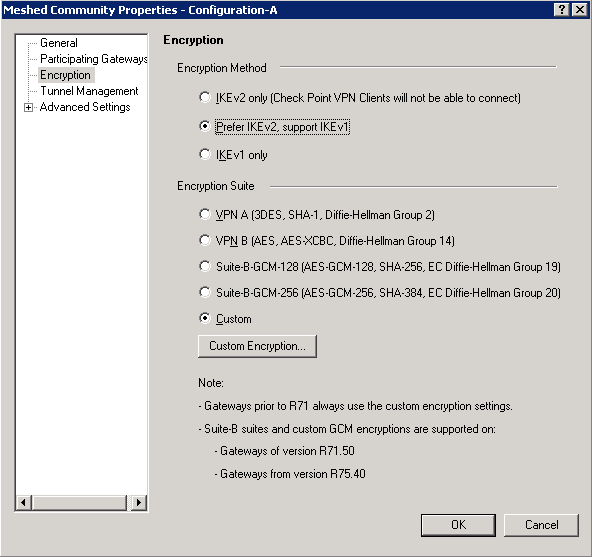
\includegraphics{checkpoint_1.png}

Either chose one of the encryption suites here, or proceed to
``Custom Encryption...'', where you can set encryption and hash for
Phase 1 and 2:

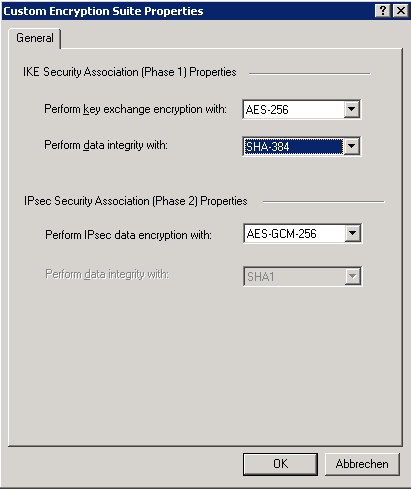
\includegraphics{checkpoint_2.png}

The Diffie-Hellman groups and Perfect Forward Secrecy Settings can be
found under ``Advanced Settings'' / ``Advanced VPN Properties'':

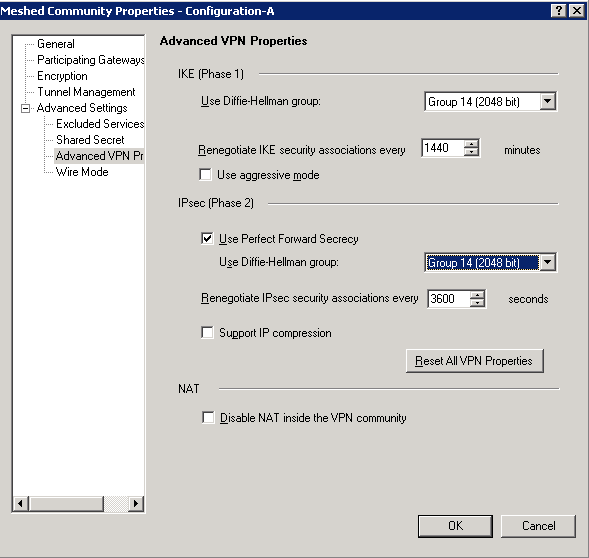
\includegraphics{checkpoint_3.png}

\item[Additional settings:]

For remote Dynamic IP Gateways, the settings are not taken from the
community, but set in the ``Global Properties'' dialog under ``Remote
Access'' / ``VPN Authentication and Encryption''. Via the ``Edit...''
button, you can configure sets of algorithms that all gateways support:

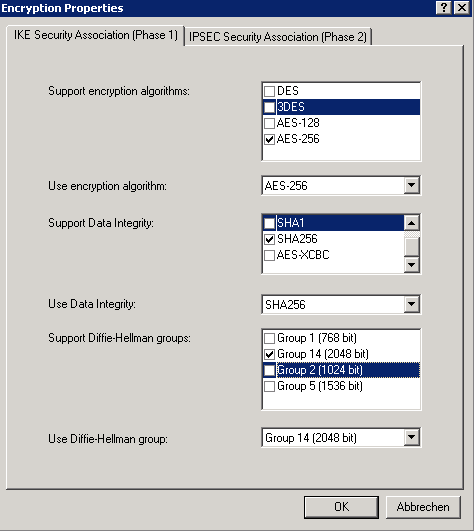
\includegraphics{checkpoint_4.png}

Please note that these settings restrict the available algorithms for
\textbf{all} gateways, and also influence the VPN client connections.

%\item[Justification for special settings (if needed):]

%\item[Limitations:]

\item[References:]\mbox{}

\begin{itemize}

\item Check Point
  \href{https://sc1.checkpoint.com/documents/R77/CP_R77_VPN_AdminGuide/html_frameset.htm}{VPN
    R77 Administration Guide} (may require a
  UserCenter account to access)

\end{itemize}

% \item[How to test:]

\end{description}


\subsubsection{OpenVPN}

\begin{description}

\item[Tested with Version:] OpenVPN 2.3.2 from Debian backports linked against openssl (libssl.so.1.0.0) 

\todo{cm: please write this subsubsection}
\todo{We suppose user uses easy-rsa which is roughly used in all HOWTO\footnote{\url{http://openvpn.net/index.php/open-source/documentation/howto.html}}}


\item[Additional settings:] \mbox{}

\paragraph{Fine tuning at installation level}

When installing an OpenVPN server instance, you are probably using {\it easy-rsa} tools to generate the crypto stuff needed.
From the directory where you will run them, you can enhance you configuration by changing the following variables in \verb|vars|:

\begin{lstlisting}[breaklines]
export KEY_SIZE=2048 
export KEY_EXPIRE=365
export CA_EXPIRE=1826
\end{lstlisting}

This will enhance the security of the key generation by using RSA keys
with a length of 2048 bits, and set a lifetime of one year for the
keys and five years for the CA certificate.

In addition, edit the \verb|pkitool| script and replace all occurences
of \verb|sha1| with \verb|sha256|, to sign the certificates with
SHA256.

\paragraph{Server Configuration}

In the server configuration file, you can select the algorithm that will be used for traffic encryption.
Based on previous recommendation established in that document, select AES with a 256 bits key in CBC mode.

Note that TLS is used only for negotiation bla bla bla...

\todo{cm: explain how openvpn crypto works; make configA/B sections/tables}

\item[Settings:] \mbox{}

% openvpn --show-ciphers
% --show-tls

\todo{cm: changelog 2.3.1: ``Switch to IANA names for TLS ciphers'' --
give both types of strings?}

\begin{lstlisting}[breaklines]
cipher AES-256-CBC   # AES

# TLS Authentication
tls-auth ta.key
tls-cipher EECDH+aRSA+AESGCM:EECDH+aRSA+SHA384:EECDH+aRSA+SHA256:EDH+CAMELLIA256:EECDH:EDH+aRSA:+SSLv3:!aNULL:!eNULL:!LOW:!3DES:!MD5:!EXP:!PSK:!SRP:!DSS:!RC4:!SEED:!AES128:!CAMELLIA128:!ECDSA:AES256-SHA

auth SHA512

reneg-bytes XXX
reneg-pkts XXX
reneg-sec XXX

\end{lstlisting}

% tls-cipher is a list, C&P the string!
% what about: TLS-DHE-RSA-WITH-AES-256-CBC-SHA
% DH params/DH key sizes

\todo{Explain a little bit tls-auth and auth directives + TEST}
\todo{also test with network-damager?}

The following ciphers are avaible and recommended\footnote{You can retrieve the list of supported algorithm on your OpenVPN installation thanks to the command {\it openvpn --show-ciphers}}
\begin{lstlisting}[breaklines]
AES-128-CBC
AES-192-CBC
AES-256-CBC
CAMELLIA-128-CBC
CAMELLIA-192-CBC
CAMELLIA-256-CBC
SEED-CBC
\end{lstlisting}


\paragraph{Client Configuration}

Client and server have to use identical configuration otherwise they can't communicate.
The {\it cipher} directive has then to be identical in both server and client configuration.

\begin{lstlisting}[breaklines]
cipher AES-256-CBC   # AES

remote-cert-tls server # http://openvpn.net/index.php/open-source/documentation/howto.html#mitm

tls-remote server.example.com

\end{lstlisting}

\todo{what about tls-auth keys/ta.key? }. 
\todo{what about auth sha512 ?}

\item[Justification for special settings (if needed):]

\item[References:] \url{http://openvpn.net/index.php/open-source/documentation/security-overview.html}

\item[How to test:]
\todo{write me please}


\end{description}


\subsubsection{PPTP}

PPTP is considered insecure, Microsoft recommends to ``use a more secure VPN
tunnel''\footnote{\url{http://technet.microsoft.com/en-us/security/advisory/2743314}}.

There is a cloud service that cracks the underlying MS-CHAPv2
authentication protocol for the price of USD~200\footnote{\url{https://www.cloudcracker.com/blog/2012/07/29/cracking-ms-chap-v2/}},
and given the resulting MD4 hash, all PPTP traffic for a user can
be decrypted.

\subsubsection{Cisco IPSec}
\todo{write this subsubsection}

\subsubsection{Juniper VPN}
\todo{write this subsubsection. AK: ask Hannes}

\subsubsection{L2TP over IPSec}
\todo{write this subsubsection}

\subsubsection{Racoon}
\todo{write this subsubsection}


\subsection{PGP/ GPG - Pretty Good Privacy}

\todo{re-work this subsection -- this is still only a draft!!}
% hack.
\gdef\currentsectionname{GPG}
\gdef\currentsubsectionname{GnuPG}

The OpenPGP protocol\footnote{\url{https://tools.ietf.org/search/rfc4880}} defines a set of asymmetric- and symmetric encryption algorithms, signature methods and compression protocols. GnuPG\footnote{\url{https://gnupg.org/}}, a FOSS implementation of the OpenPGP standard, is widely used for mail encryption.
 
GnuPG signs a message (SHA-2, RIPEMD or SHA-1), encrypts it symmetrically (AES, CAMELLIA, TWOFISH, BLOWFISH, 3DES, CAST5 or IDEA) and encrpts the symmetric key and the hash with Bob's public key asymmetrically (RSA, ELG, DSA, ECDH, ECDSA or EDDSA).

Research on SHA-1 conducted back in 2005\footnote{\url{https://www.schneier.com/blog/archives/2005/02/sha1\_broken.html}} as well as the first practical successful collision in early 2017\footnote{\url{https://shattered.io/}} has made clear that collision attacks are a real threat to the security of the SHA-1 hash function. Since SHA-1 is defined as a must implementation by the OpenPGP specification, GnuPG is still using it. Currently settings should be adapted to preferably avoid using SHA-1. 

When using GnuPG, there are a couple of things to take care of:
\begin{itemize*}
  \item keylengths (see section \ref{section:keylengths})
  \item randomness (see section \ref{section:RNGs})
  \item preference of symmetric encryption algorithm (see section \ref{section:CipherSuites})
  \item preference of hash function (see section \ref{section:CipherSuites})
\end{itemize*}

Properly dealing with key material, passphrases and the web-of-trust is outside of the scope of this document. The GnuPG website\footnote{\url{http://www.gnupg.org}} has a good tutorial on PGP.

This \href{https://www.debian-administration.org/users/dkg/weblog/48}{Debian How-to}\footnote{\url{https://www.debian-administration.org/users/dkg/weblog/48}} is a great resource on upgrading your old PGP key as well as on safe default settings. This section is built based on the Debian How-to.

\subsubsection{Hashing}
Avoid SHA-1 by prefering better hashing methodes. GnuPG. Edit \$HOME/.gnupg/gpg.conf:

\configfile{gpg.conf}{208-210}{Digest selection in GnuPG}

Before you generate a new OpenPGP key, make sure there is enough entropy available (see subsection \ref{subsec:RNG-linux}).

\subsection{Key Generation}
\gdef\currentsectionname{GPG}
\gdef\currentsubsectionname{GnuPG}
Because of lack of forward secrecy\ac{PFS} in OpenPGP it is preferable to use large asymmetric keys for long term
communication protection. A RSA key of 8192 bits should provide enough confidentiallity for the next 15+ years\footnote{\url{https://www.keylength.com}}.

\configfile{new-key-generation.txt}{}{New key generation with GnuPG version 2.1}

\configfile{params.txt}{}{Paramters for key generation with GnuPG version 2.1}

\subsection{ECC - Ellyptic Curve Cryptography}
Since the realease of GnuPG version 2.1 end-2014\footnote{\url{https://www.gnupg.org/faq/whats-new-in-2.1.html}} ECC is supported. Older versions though are still widely used therefore ECC is not yet applicable in practice. 

%\subsubsection{PGP / GPG Operations}

%% Ciphering - Unciphering operations
%%% TOO COMPLEX. Make a pointer to a good GPG tutorial

%% Signing / checking signatures
%%% TOO COMPLEX. Make a pointer to a good GPG tutorial

%\subsubsection{Trusted Keys}

%%Explain that a key by himself is not trustable.  Chain of trust principle.

%%% TOO COMPLEX. Make a pointer to a good GPG tutorial

%\subsection{Available implementations and mails plugins}

%% Microsoft Windows (Symantec for Outlook? GnuPG + ....)
%%% TOO COMPLEX. Make a pointer to a good GPG tutorial

%% Linux (GnuPG + Enigmail for Thunderbird)

%%% TOO COMPLEX. Make a pointer to a good GPG tutorial
%% Mac OS X (GnuPG + GPGMail)
%%% TOO COMPLEX. Make a pointer to a good GPG tutorial




\subsection{seclayer-tcp}
\todo{Ramin: please write this section or ask Posch}
For the austrian citizen card....

\begin{verbatim}
seclayer-tcp    3495/udp    # securitylayer over tcp
seclayer-tcp    3495/tcp    # securitylayer over tcp
\end{verbatim}


\subsection{IPMI, ILO and other lights out management solutions}


We \textbf{strongly} recommend that any remote management system for servers such as ILO, IPMI and similar never be connected to a public IP address.
Consider creating a management VLAN and access that only via a VPN.


\subsection{SIP}
\todo{AK: ask Klaus. Write this section, Klaus??? }

\subsection{Instant Messaging Systems}
\subsubsection{XMPP / Jabber}
\todo{ts: Describe ejabberd configuration. Reference to Peter`s manifesto https://github.com/stpeter/manifesto}
\subsubsection{IRC}

%%\subsection{Database Systems}
% This list is based on : http://en.wikipedia.org/wiki/Relational_database_management_system#Market_share

\subsubsection{Oracle}
\todo{write this}

\subsubsection{SQL Server}
\todo{write this}




\subsubsection{MySQL}

\begin{description}
\item[Tested with Version:] Debian 7.0 and MySQL 5.5

\item[Settings:] \mbox{}

\paragraph*{my.cnf}\mbox{}\\

\begin{lstlisting}[breaklines]
[mysqld]
ssl
ssl-ca=/etc/mysql/ssl/ca-cert.pem
ssl-cert=/etc/mysql/ssl/server-cert.pem
ssl-key=/etc/mysql/ssl/server-key.pem
ssl-cipher=EECDH+aRSA+AESGCM:EECDH+aRSA+SHA384:EECDH+aRSA+SHA256:EDH+CAMELLIA256:EECDH:EDH+aRSA:+SSLv3:!aNULL:!eNULL:!LOW:!3DES:!MD5:!EXP:!PSK:!SRP:!DSS:!RC4:!SEED:!AES128:!CAMELLIA128:!ECDSA:AES256-SHA
\end{lstlisting}

\item[Additional settings:]


\item[Justification for special settings (if needed):]

% in case you have the need for further justifications why you chose this and that setting or if the settings do not fit into the standard Variant A or Variant B schema, please document this here

\item[References:]
+{\small \url{https://dev.mysql.com/doc/refman/5.5/en/ssl-connections.html}}


% add any further references or best practice documents here

\item[How to test:]

After restarting the server run the following query to see if the ssl settings are correct:
\begin{lstlisting}[breaklines]
show variables like '%ssl%';
\end{lstlisting}


\end{description}






\subsubsection{DB2}
\todo{write this}





\subsubsection{Postgresql}

\begin{description}
\item[Tested with Version:] Debian 7.0 and PostgreSQL 9.1

\item[References:]

It's recommended to read 

{\small \url{http://www.postgresql.org/docs/current/static/runtime-config-connection.html#RUNTIME-CONFIG-CONNECTION-SECURITY}}
{\small \url{http://www.postgresql.org/docs/current/static/ssl-tcp.html}}
{\small \url{http://www.postgresql.org/docs/current/static/auth-pg-hba-conf.html}}

\item[Settings:] \mbox{}


To start in SSL mode the server.crt and server.key must exist in the server's data directory \$PGDATA. 

Starting with version 9.2, you have the possibility to set the path.

\begin{lstlisting}[breaklines]
ssl_key_file = '/your/path/server.key'
ssl_cert_file = '/your/path/server.crt'
ssl_ca_file = '/your/path/root.crt'
\end{lstlisting}

\paragraph*{postgresql.conf}\mbox{}\\

\begin{lstlisting}[breaklines]
#>=8.3
ssl = on 
ssl_ciphers = 'EECDH+aRSA+AESGCM:EECDH+aRSA+SHA384:EECDH+aRSA+SHA256:EDH+CAMELLIA256:EECDH:EDH+aRSA:+SSLv3:!aNULL:!eNULL:!LOW:!3DES:!MD5:!EXP:!PSK:!SRP:!DSS:!RC4:!SEED:!AES128:!CAMELLIA128:!ECDSA:AES256-SHA'
\end{lstlisting}



\item[How to test:]
To test your ssl settings, run psql with the sslmode parameter:
\begin{lstlisting}[breaklines]
psql "sslmode=require host=postgres-server dbname=database" your-username
\end{lstlisting}

\end{description}




\subsubsection{Informix}
\todo{write this}


%hack.
\gdef\currentsectionname{Proxies}
%%\subsection{Intercepting proxy solutions and reverse proxies}

Within enterprise networks and corporations with increased levels of paranoia or at least some defined security requirements it is common \textbf{not} to allow direct connections to the public internet.

For this reason proxy solutions are deployed on corporate networks to intercept and scan the traffic for potential threats within sessions.

For encrypted traffic there are four options:

\begin{itemize*}
  \item Block the connection because it cannot be scanned for threats.
  \item Bypass the threat-mitigation and pass the encrypted session to the client, which results in a situation where malicious content is transferred directly to the client without visibility to the security system.
  \item Intercept (i.e. terminate) the session at the proxy, scan there and re-encrypt the session towards the client (effectively MITM).
  \item Deploy special Certificate Authorities to enable Deep Packet Inspection on the wire.
\end{itemize*}

While the latest solution might be the most "up to date", it arises a new front in the context of this paper, because the most secure part of a client's connection could only be within the corporate network, if the proxy-server handles the connection to the destination server in an insecure manner.

Conclusion: Don't forget to check your proxy solutions SSL-capabilities. Also do so for your reverse proxies!

%% ---------------------------------------------------------------------- 
% who was the author of this section?
% can we have this either tested or removed?
%\subsection{Squid}
%As of squid-3.2.7 (01 Feb 2013) there is support for the OpenSSL NO\_Compression option within squid config (CRIME attack) and if you combine that in the config file, with an enforcement of the server cipher preferences (BEAST Attack) you are safe.
%
%
%\todo{UNTESTED!}
%\configfile{squid.conf}{1363-1363,1379-1379}{Cipher selection and SSL options in Squid}
%%% http://forum.pfsense.org/index.php?topic=63262.0
%%\todo{UNTESTED!}
%% see squid.conf, repeating the options here does not help.
%\todo{Patch here? Definitely working for 3.2.6!}
%For squid Versions before 3.2.7 use this patch against a vanilla source-tree:
%\begin{lstlisting}
%--- support.cc.ini      2013-01-09 02:41:51.000000000 +0100
%+++ support.cc  2013-01-21 16:13:32.549383848 +0100
%@@ -400,6 +400,11 @@
%         "NO_TLSv1_2", SSL_OP_NO_TLSv1_2
%     },
% #endif
%+#ifdef SSL_OP_NO_COMPRESSION
%+    {
%+        "NO_Compression", SSL_OP_NO_COMPRESSION
%+    },
%+#endif
%     {
%         "", 0
%     },
%\end{lstlisting}
%
%
%% ---------------------------------------------------------------------- 
\subsection{Bluecoat}
%% https://kb.bluecoat.com/index?page=content&id=KB5549
\subsubsection{Tested with Versions}
\begin{itemize*}
  \item SGOS 6.5.x
\end{itemize*}

BlueCoat Proxy SG Appliances can be used as forward and reverse proxies. The reverse proxy feature is rather under-developed, and while it is possible and supported, there only seems to be limited use of this feature "in the wild" - nonetheless there are a few cipher suites to choose from, when enabling SSL features.

\paragraph*{Only allow TLS 1.0,1.1 and 1.2 protocols:}
~
\begin{lstlisting}
$conf t
$(config)ssl
$(config ssl)edit ssl-device-profile default
$(config device-profile default)protocol tlsv1 tlsv1.1 tlsv1.2
  ok
\end{lstlisting}

\paragraph*{Select your accepted cipher-suites:}
~
\begin{lstlisting}
$conf t
Enter configuration commands, one per line.  End with CTRL-Z.
$(config)proxy-services
$(config proxy-services)edit ReverseProxyHighCipher
$(config ReverseProxyHighCipher)attribute cipher-suite
Cipher#  Use        Description        Strength
-------  ---  -----------------------  --------
      1  yes            AES128-SHA256      High
      2  yes            AES256-SHA256      High
      3  yes               AES128-SHA    Medium
      4  yes               AES256-SHA      High
      5  yes       DHE-RSA-AES128-SHA      High
      6  yes       DHE-RSA-AES256-SHA      High
               [...]
     13  yes          EXP-RC2-CBC-MD5    Export

Select cipher numbers to use, separated by commas: 2,5,6
  ok
\end{lstlisting}

The same protocols are available for forward proxy settings and should be adjusted accordingly:
In your local policy file add the following section:
\begin{lstlisting}
<ssl>
    DENY server.connection.negotiated_ssl_version=(SSLV2, SSLV3)
\end{lstlisting}

Disabling protocols and ciphers in a forward proxy environment could lead to unexpected results on certain (misconfigured?) webservers (i.e. ones accepting only SSLv2/3 protocol connections)


%% ---------------------------------------------------------------------- 
\subsection{HAProxy}
% See http://www.haproxy.org/

HAProxy can be used as loadbalancer and proxy for TCP and HTTP-based applications. Since version 1.5 it supports SSL and IPv6.

\subsubsection{Tested with Versions}
\begin{itemize*}
  \item HAProxy 1.5.11 with OpenSSL 1.0.1e on Debian Wheezy
\end{itemize*}

\subsubsection{Settings}
\configfile{haproxy.cfg}{1-4}{global configuration}
\configfile{haproxy.cfg}{21-25}{frontend configuration}
\configfile{haproxy.cfg}{27-33}{backend configuration}


%% ---------------------------------------------------------------------- 
\subsection{Pound}
% See http://www.apsis.ch/pound
% See https://help.ubuntu.com/community/Pound

\subsubsection{Tested with Versions}
\begin{itemize*}
  \item Pound 2.6
\end{itemize*}

\subsubsection{Settings}
\configfile{pound.cfg}{31}{HTTPS Listener in Pound}


%% ---------------------------------------------------------------------- 
\subsection{stunnel}
% See https://www.stunnel.org/

\subsubsection{Tested with Versions}
\begin{itemize*}
  \item stunnel 4.53-1.1ubuntu1 on Ubuntu 14.04 Trusty with OpenSSL 1.0.1f, without disabling Secure Client-Initiated Renegotiation
  \item stunnel 5.02-1 on Ubuntu 14.04 Trusty with OpenSSL 1.0.1f
  \item stunnel 4.53-1.1 on Debian Wheezy with OpenSSL 1.0.1e, without disabling Secure Client-Initiated Renegotiation
\end{itemize*}

\subsubsection{Settings}
\configfile{stunnel.conf}{48-55}{HTTPS Listener in Pound}

\subsubsection{Additional information}
Secure Client-Initiated Renegotiation can only be disabled for stunnel versions >= 4.54, when the renegotiation parameter has been added (See changelog).

\subsubsection{References} 
\begin{itemize*}
  \item stunnel documentation: \url{https://www.stunnel.org/static/stunnel.html}
  \item stunnel changelog: \url{https://www.stunnel.org/sdf_ChangeLog.html}
\end{itemize*}


\subsubsection{How to test} 
See appendix \ref{cha:tools}

 



%%% Local Variables: 
%%% mode: latex
%%% TeX-master: "applied-crypto-hardening"
%%% End: 

\section{Tools}

This section lists tools for checking the security settings.

\subsection{SSL \& TLS}

Check your browser's ssl capabilities: \url{https://cc.dcsec.uni-hannover.de/}


ssllabs.com offers a great way to check your webserver for misconfigurations. See \url{https://www.ssllabs.com/ssltest/}.
Furthermore, ssllabs.com has a good best practices tutorial, which focuses on avoiding the most common mistakes in SSL.
See: \url{https://www.ssllabs.com/downloads/SSL_TLS_Deployment_Best_Practices_1.3.pdf}
%% this breaks my pdf converter hmm

\url{http://tls.secg.org} is a tool for testing interoperability of HTTPS implementations for ECC cipher suites.

\url{http://sourceforge.net/projects/sslscan} connects to a given SSL
service and shows the cipher suites that are offered.

\url{http://checktls.com} is a tool for testing arbitrary TLS services. 

\url{https://github.com/iSECPartners/sslyze} Fast and full-featured SSL scanner

\subsection{Keylength}

\url{http://www.keylength.com} comprehensive online resource for comparison of keylenghts according to common recommendatons and standards in cryptography.

\subsection{RNGs}

%% NOTE: should we merge that with chapter 6.6??
\begin{itemize}
\item \href{http://www.fourmilab.ch/random/}{ENT} is a pseudo random number generator sequence tester.  
\item \href{http://www.issihosts.com/haveged/}{HaveGE} is a tool which increases the Entropy of the Linux random number generator devices. It is based on the HAVEGE algorithm. \url{http://dl.acm.org/citation.cfm?id=945516}
\end{itemize}




\chapter{Further research}
\label{cha:further-research}
The following is a list of services, software packages, hardware devices or protocols that we considered documenting but either did not manage to document yet or might be able to document later. We encourage input from the Internet community. 

\begin{multicols}{3}
\begin{itemize}
\item whatsapp (might be problematic\\ since a user/admin can't change anything)
\item Lync
\item Skype (might be problematic since a user/admin can't change anything)
\item Wi-Fi APs, 802.1X
\item Tomcat
\item SIP 
\item SRTP 
\item DNSSec (mention BCPs) 
\item DANE
\item TOR 
\item S/Mime (check are there any BCPs? )
\item TrueCrypt, LUKS, FileVault
\item AFS 
\item Kerberos 
\item NNTP 
\item NTPs tlsdate 
\item BGP / OSPF 
\item SILC
\item LDAP
\item seclayer-tcp
\item Commerical network equipment vendors
\item RADIUS 
\item Moxa , APC, und co... ICS . Ethernet to serial 
\item telnet (only sensible reocmmendation: \emph{DON't!!})
\item rsyslog 
\item v6 spoofing (look at work by Ferndo Gont, Marc Heuse, et. al.)
\item tinc
\item racoon
\item l2tp
\item rsync 
\item telnets 
\item ftps 
\item webmin (probably the same recommendations as with Apache apply, but where does that need to be configured?)
\item plesk (same as webmin)
\item phpmyadmin (same as webmin)
\item DSL modems (where to start?)
\item UPnP, natPmp 
\item SAML federated auth providers \footnote{e.g., all the REFEDS folks (\url{https://refeds.org/})), including InCommon (\url{http://www.incommon.org/federation/metadata.html}
  \url{https://wiki.shibboleth.net/confluence/display/SHIB2/TrustManagement} }
\item Microsoft SQL Server
\end{itemize}
\end{multicols}

%%% Local Variables: 
%%% mode: latex
%%% TeX-master: "applied-crypto-hardening"
%%% End: 

\chapter{Links}
\label{cha:links}
%% NOTE: this should re restructured...

\begin{itemize*}
  \item IANA official list of Transport Layer Security (TLS) Parameters: \url{https://www.iana.org/assignments/tls-parameters/tls-parameters.txt}
  \item SSL cipher settings: \url{http://www.skytale.net/blog/archives/22-SSL-cipher-setting.html}
  \item Elliptic curves and their implementation (04 Dec 2010): \url{https://www.imperialviolet.org/2010/12/04/ecc.html}
  \item A (relatively easy to understand) primer on elliptic curve cryptography: \url{http://arstechnica.com/security/2013/10/a-relatively-easy-to-understand-primer-on-elliptic-curve-cryptography}
  \item Duraconf, A collection of hardened configuration files for SSL/TLS services (Jacob Appelbaum's github): \url{https://github.com/ioerror/duraconf}
  \item Attacks on SSL a comprehensive study of BEAST, CRIME, TIME, BREACH, LUCKY 13 \& RC4 Biases: \url{https://www.isecpartners.com/media/106031/ssl_attacks_survey.pdf}
  \item EFF How to deploy HTTPS correctly: \url{https://www.eff.org/https-everywhere/deploying-https}
  \item Bruce Almighty: Schneier preaches security to Linux faithful (on not recommending to use Blowfish anymore in favor of Twofish): \url{https://www.computerworld.com.au/article/46254/bruce_almighty_schneier_preaches_security_linux_faithful/?pp=3}
  \item Implement FIPS 183-3 for DSA keys (1024bit constraint): \url{https://bugzilla.mindrot.org/show_bug.cgi?id=1647}
  \item Elliptic Curve Cryptography in Practice: \url{http://eprint.iacr.org/2013/734.pdf}
  \item Factoring as a Service: \url{http://crypto.2013.rump.cr.yp.to/981774ce07e51813fd4466612a78601b.pdf}
  \item Black Ops of TCP/IP 2012: \url{http://dankaminsky.com/2012/08/06/bo2012/}
  \item SSL and the Future of Authenticity, Moxie Marlinspike - Black Hat USA 2011: \url{https://www.youtube.com/watch?v=Z7Wl2FW2TcA}
  \item ENISA - Algorithms, Key Sizes and Parameters Report (Oct.'13) \url{http://www.enisa.europa.eu/activities/identity-and-trust/library/deliverables/algorithms-key-sizes-and-parameters-report}
  \item Diffie-Hellman Groups \url{http://ibm.co/18lslZf}
  \item Diffie-Hellman Groups standardized in RFC3526~\cite{rfc3526} \url{https://datatracker.ietf.org/doc/rfc3526/}
  \item ECC-enabled GnuPG per RFC6637~\cite{rfc6637} \url{https://code.google.com/p/gnupg-ecc}
  \item TLS Security (Survey + Lucky13 + RC4 Attack) by Kenny Paterson \url{https://www.cosic.esat.kuleuven.be/ecc2013/files/kenny.pdf}
  \item Ensuring High-Quality Randomness in Cryptographic Key Generation \url{http://arxiv.org/abs/1309.7366v1}
  \item Wikipedia: Ciphertext Stealing \url{https://en.wikipedia.org/wiki/Ciphertext_stealing}
  \item Wikipedia: Malleability (Cryptography) \url{https://en.wikipedia.org/wiki/Malleability_(cryptography)}
  \item Ritter's Crypto Glossary and Dictionary of Technical Cryptography \url{http://www.ciphersbyritter.com/GLOSSARY.HTM}
\end{itemize*}

\section{Suggested Reading}
\label{section:Suggested_Reading}
This section contains suggested reading material.

\begin{itemize}
	\item Cryptography Engineering: Design Principles and Practical Applications, Ferguson, N. and Schneier, B. and Kohno, T. (ISBN-13: 978-0470474242)
	\item Security Engineering: A Guide to Building Dependable Distributed Systems, Anderson, R.J. (ISBN-13: 978-0470068526)
	\item Applied cryptography: protocols, algorithms, and source code in C, Schneier, B. (ISBN-13: 978-0471117094)
	\item Guide to Elliptic Curve Cryptography, Hankerson, D. and Vanstone, S. and Menezes, A.J. (ISBN-13: 978-0387952734)
	\item A Introduction To The Theory of Numbers, Godfrey Harold Hardy, E. M. Wrigh (ISBN-13: 978-0199219865)
	\item Malicious Cryptography: Exposing Cryptovirology, Young A., Yung, M. (ISBN-13: 978-0764549755)
\end{itemize}

%% should we include bibtex instead? can be downloaded from books.google.com

%\section{Acknowledgements}

%% add something useful

\section{Reviewers}

We would like to express our thanks to the following reviewers (in alphabetical order):

Horenbeck, Maarten;
Lenzhofer, Stefan;
Schreck, Thomas; 



\bibliography{security}


\end{document}
